% The paper: the Study 1 report extended with Study 2's results. Compile with pdflatex + bibtex (plainnat)
% on TeX Live or MiKTeX. Sections 1 to 6, the Study 1 limitations, the follow-up paragraph, the
% reproducibility paragraph, the author's statement and Appendices A to D are the report's own text, read
% from the shared files under shared/ that main.tex also reads; the Study 2 sections are under sections/.
% Every number traces to a file and a command listed in sources.md and is asserted by check_numbers.py.
\documentclass[10pt]{article}
\usepackage[a4paper,margin=24mm]{geometry}
\usepackage{amsmath}
\usepackage{booktabs}
\usepackage{graphicx}
\usepackage[hyphens]{url}
\usepackage[numbers,sort&compress]{natbib}
\usepackage[colorlinks=true,allcolors=blue]{hyperref}

\graphicspath{{figures/}}
\newcommand{\lm}{\texttt{local\_mean\_28}}
\newcommand{\aets}{\texttt{autoets\_weekly}}
\newcommand{\qs}{QScore9}
\newcommand{\hc}{\texttt{hurdle\_count\_28}}
% DOI: the author reserves the DOI on posting day and replaces the text below.
\newcommand{\reportdoi}{DOI to be filled on posting day}

\title{Zero-shot foundation models on sparse daily counts:\\a registered re-evaluation on GitHub stars and a
registered occurrence test on npm downloads}
\author{Victor Prchlik}
\date{Paper version, October 2026 \\ \small \reportdoi}

\begin{document}
\maketitle

\begin{abstract}
We ask whether zero-shot time-series foundation models improve probabilistic forecasts of sparse daily
counts, and test one mechanism behind the answer. Study 1 is a registered re-evaluation on daily GitHub
star counts after an audit of a first version (protocol commit \texttt{5f01769}, 2026-09-12): 300
repositories sampled from a frame of 148,550, three frozen models (Chronos-2, TimesFM 3, TimesFM 2.5)
against a 28-day local mean and weekly AutoETS, a nine-decile quantile score, 18 declared comparisons.
Against the local mean the mean difference favors the models in every cell and its bootstrap interval
excludes zero in five of nine, but the typical repository favors the reference: the models score lower on
46 to 89 of 300 repositories and the signed-rank test rejects in all nine cells on the reference's side.
Against AutoETS both summaries favor the models, consistent with its 80 percent intervals covering about 99
percent of target days. Study 2, registered after those results (commit \texttt{df55867}, 2026-09-14), asks
whether replacing a frozen model's own zero mass with a context-only occurrence probability, keeping its
completed positive law, lowers the score, and whether that positive law beats a fixed count hurdle. On a
hash-sampled npm download panel of 209 series (100 dense, 100 sparse, 9 very sparse) no comparison favors
the substitution and two of six reject against it; the model's positive law beats the count hurdle in all
six cells. On a registered 540-series synthetic grid five of six tests reject, all
against the substitution. One series at 7.6 million downloads a day carries every npm mean, so the medians
and rank tests describe the typical series; a post-hoc sensitivity to three zero days served by the source
changes no mechanism conclusion. A literature re-check allows the claim of this registered combination on
daily attention and adoption counts, and nothing broader.
\end{abstract}

\section{Introduction}

The question is whether zero-shot time-series foundation models improve probabilistic forecasts of the daily
number of new stars a GitHub repository receives. These series are counts, most days are zero for most
repositories, activity arrives in bursts tied to releases and external attention, and the panel one can
observe is survivor-biased: a repository that was deleted or made private has no history to fetch. Public
forecasting benchmarks are mostly smooth, seasonal, positive series, so this kind of data is a hard case for
zero-shot forecasting. The practical question is whether such a model is worth running at all on a sparse
count series, or whether a trailing mean does as well.

The story of this report is in four parts. A first version of the study, built in June and July 2026, found
two foundation models ahead of classical baselines on mean CRPS in every cell of its design. An adversarial
audit on 2026-07-12 found no code defect that invalidated the aggregate comparison, but two design flaws that
could not be fixed by rewriting prose: the cohorts had been selected on outcomes not available at forecast
time, and the evaluation windows mostly tested post-peak decay. We registered a redesign on 2026-09-12, before
any target was fetched, and ran it on 2026-09-13 without change. The revised result is less flattering and is
reported with the same care: the models win on the mean against a 28-day local mean, lose on most individual
repositories, and win on both summaries against a weekly AutoETS whose intervals are far too wide. A post-hoc
accounting of the saved run, labeled as such, says where the mean gain comes from.

This is not the first observation that an aggregate gain can coexist with a minority win rate. A July 2026
quick-commerce study found TimesFM's pooled gains concentrated in high-turnover items while it won a minority
of item-rounds on lumpy demand \citep{kim2026}, and a marketplace-panel study showed the aggregate and
per-series rankings of five zero-shot foundation models reversing on M5 \citep{islam2026}. Frozen foundation
models have also been evaluated on sparse daily counts before: twelve of them, the three used here among
them, on five sparse panels as an event-ranking task without a proper score \citep{schoess2026}; and TimesFM 3
on simulated intermittent demand, where its nine-decile pinball loss was no better than the history's
empirical deciles \citep{ebrahim2026}, a finding consistent with the typical-repository result reported here.
Earlier evaluations on cloud workloads found simple baselines ahead \citep{toner2025}, and the Chronos and
TimesFM papers themselves report benchmark results that include count-like series without a zero-day
diagnosis \citep{ansari2024, das2023}. Benchmark practice has moved toward reporting win rates alongside
relative errors \citep{fevbench2026}, and the forecast-evaluation literature warns against ratio metrics that
silently drop series \citep{hewamalage2023}. Star-count prediction on GitHub has been studied as a regression
on popular repositories \citep{borges2016}, and a live benchmark scores daily new stargazers on the 400
most-starred repositories \citep{garza2026}; the present design samples from a population rather than from
the popular. What this report adds is a registered, population-sampled, repository-clustered probabilistic
evaluation whose every number traces to a saved file.


This paper extends that report. Sections~1 to~6 are the report's text, unchanged in meaning: this
introduction, the first version and its audit, the registered design, the achieved panel, the results and
the post-hoc accounting.
Sections~7 to~10 add Study 2, registered after Study 1's results were seen and run on data declared for the
purpose: its question, its design, the achieved npm panel, and the results of its external and synthetic
components. Section~11 reads the two studies together, Section~12 extends the limitations, Section~13 says
what is registered and not run, and Section~14 extends the reproducibility statement. The Study 1 report
stands on its own as a posted document; nothing here changes its numbers or its claims.

\section{Version 1 and the audit}

Version 1 ingested 208 repositories found by three GitHub Search API queries (recently created and already
high-starred; old, moderate and recently maintained; not pushed in years), giving 414,271 daily rows from
2008-11-13 to 2026-06-22, of which 179 repositories had at least 270 days of history (41, 69 and 69 in the
three cohorts). The backtest used an expanding context starting 180 days after the first star, a 30-day step,
at most eight windows per repository, horizons of 7, 30 and 90 days, and 200 predictive trajectories per
model. Four classical baselines (horizon-dependent seasonal naive, linear trend, damped ETS, LightGBM) and two
foundation models, Chronos-2 and TimesFM-2.5, were scored by empirical CRPS. Both foundation models had lower
mean CRPS than every original baseline in all nine cohort-by-horizon cells; in the ``breakout'' cohort the
foundation models scored 6.2 to 8.5 against 11.2 to 28.0 for the baselines.

The audit of 2026-07-12 found no code defect that invalidated the aggregate six-model comparison; every
summary field recomputed from the saved artifact. It found two design flaws that invalidated the original
claims:
\begin{enumerate}
\item \emph{Outcome-conditioned cohorts.} ``Breakout'' was selected for already having many stars, ``dead''
  for later inactivity, ``steady'' for later maintenance. None of these labels was available at forecast
  time. The ``dead'' cohort's evaluation windows had a median of 5.02 stars per day and only 7.7 percent zero
  days; it was not dead when evaluated.
\item \emph{Post-peak windows.} The global peak preceded the evaluated span for 78.0 percent of breakout
  repositories; only 12.2 percent peaked inside it. The study tested the forecasting of post-viral decay, not
  of shocks.
\end{enumerate}
After the audit added a 28-day local mean on identical windows, the foundation models still had the lower
mean in every cell (Appendix Table~\ref{tab:v1}), but the per-repository win rate against it fell to between
40.6 and 80.5 percent, and the audit put the share of positive gain held by the five largest positive
contributors at roughly 30 to 77 percent depending on the cell, a figure it tied to no named reference. The
audit also listed what version 1 had to disclose (Appendix~\ref{app:v1}). Its prescription, freeze and
pre-register, context-only labels, trailing non-overlapping windows with a common endpoint, strong
pre-registered baselines, native quantile metrics, repository-clustered inference, and a prospective
post-release cohort as the contamination control, became the specification of version 2; the cohort is
registered and not yet run (Section~\ref{sec:notrun}). Every version 1 number in this report is quoted from
the preserved version 1 documents, not recomputed; the version 1 artifacts are on a computer the author no
longer uses.


\section{The registered design}

The protocol was registered at commit \texttt{5f01769b6be4c32814befdd7cc3395b6dcc386ed} on 2026-09-12,
before any target history was fetched; the registered file's SHA-256 is
\texttt{dfe2f4adf5c3fdafaa6f2716ae7c19cd4d52577497041c13b763ba06540f65c5}. The run's gate verified those
exact bytes. Nothing in the protocol changed after results were seen; later changes are dated additions at its
end. What follows is the design in brief; Appendix~\ref{app:design} gives the count source and its
validation, the calendar, the regime rules, the model pins, the score and the inference settings as
registered.

The question is whether zero-shot foundation models improve probabilistic forecasts of daily GitHub
star-history counts relative to \lm{} and weekly AutoETS on a panel selected by day-90 activity and
fetch-time availability; the hypothesis predicts lower repository-level \qs{} for the foundation models, and
null, adverse, mixed and imprecise results receive the same reporting. The frame is every repository created
from 2023-01-01 to 2025-02-21 (UTC) with at least 20 GH Archive WatchEvents over the creation day and the
following 89 days, in three day-90 strata (20 to 99, 100 to 999, at least 1,000 events). Within each stratum
the frame is placed in a seeded random order (selection seed 20260913), frozen before retrieval; the walk
stops at 100 repositories with complete retrieved histories, with every skip and its reason logged, and
acceptance depends on retrieval completeness only. Daily counts come from GitHub's star-history endpoint,
from creation through the common endpoint 2026-08-31, binned to America/Los\_Angeles days after an hourly
validation against GH Archive; the target is the surviving-star daily history as retrieved in September
2026. Three cutoffs, 2025-12-05, 2026-03-05 and 2026-06-03, partition the trailing 270 days into
non-overlapping 90-day windows; horizons of 7, 30 and 90 days share each cutoff. Three context-only regime
labels are descriptive. Three frozen foundation models at pinned revisions (Chronos-2, TimesFM 3, TimesFM
2.5) are compared with two primary references, \lm{}, the mean of the last 28 context days with empirical
context-level draws, and \aets{}, AutoETS with season length 7 and native intervals; thirteen secondary
baselines add no test. The score is \qs{}, twice the mean pinball loss over the nine deciles and the target
days, a proper score for the nine quantiles. Window scores are averaged within repository and horizon,
repositories are weighted equally, and each of the 18 declared comparisons (three models, two references,
three horizons) reports the mean paired difference with a repository-bootstrap interval, the median
difference and a two-sided Wilcoxon signed-rank test, with one Benjamini-Hochberg adjustment at $q = 0.05$
over the 18 tests.


\section{The achieved panel}

The frame held 148,550 eligible repositories: 100,687 in the 20 to 99 stratum, 46,811 in 100 to 999, and
1,052 in the 1,000-plus stratum (Table~\ref{tab:panel}). The seeded walk accepted 100 per stratum and skipped
470 repositories, all because the stable ID no longer resolved to a public repository at fetch time (466 with
HTTP 404) or was forbidden (4 with HTTP 403). The panel is therefore repositories still public in September
2026 with complete retrievable histories; equal repository weighting describes this panel, not all of GitHub.
The daily signal holds 289,316 repository-days with every Los Angeles calendar day from creation through
2026-08-31 observed; no missing bin was imputed. The panel is evaluated in its mature phase: the creation
dates run from 2023-01-02 to 2025-02-19, so every repository was created at least nine months before the
first cutoff, and nothing here is a launch forecast.

\begin{table}[t]
\centering\footnotesize
\caption{The achieved panel by day-90 stratum: the frame size, the accepted and skipped counts, the median
and the 10th and 90th percentiles of the survivor ratio, the number of repositories with no star from
2026-06-03 to 2026-08-31, and the median star count over those 90 days. The survivor ratio divides the
endpoint's first 90 Los Angeles days by the gross archive count over the UTC creation day and the next 89
days; the two calendars differ, so the ratio is a diagnostic, not an exact retention rate. Skips are
repositories encountered before the stratum's stop.}
\label{tab:panel}
\begin{tabular}{lrrrrrrrr}
\toprule
Stratum & Frame & Accepted & Skipped & Ratio median & P10 & P90 & Zero, last 90 & Median, last 90 \\
\midrule
20--99 & 100,687 & 100 & 98 & 0.968 & 0.723 & 1.075 & 52 & 0 \\
100--999 & 46,811 & 100 & 348 & 1.004 & 0.885 & 1.079 & 22 & 4 \\
1000+ & 1,052 & 100 & 24 & 1.006 & 0.914 & 1.049 & 1 & 39 \\
\bottomrule
\end{tabular}
\end{table}

Over the 900 repository-cutoff windows, the context-only regime labeler assigned 320 windows from 140
repositories to ``inactive recently'', 572 windows from 228 repositories to ``other active'', and 8 windows
from 7 repositories to ``recent surge''. The surge regime is too thin to say anything about bursts, and the
report does not try.

The registered run started 2026-09-13 07:54 UTC at implementation commit
\texttt{ca67dd22ea49377ee1fd074aed57b4b7460c84f1} after the signed readiness review, and completed in
18,662 seconds (5 hours and 11 minutes) with 48,600 forecast rows (300 repositories, 3 cutoffs, 3 horizons,
18 models), no failed window and no resume. The integrity check recomputed every score and verified all 300
checkpoint hashes.


\section{Results}
\label{sec:results}

Tables~\ref{tab:lm} and~\ref{tab:ae} give the 18 declared comparisons, one table per reference, each with the
mean difference and its interval, the median difference, the number of repositories where the model's \qs{}
is lower, the strict win fraction and the adjusted $p$-value side by side. Figure~\ref{fig:paired} shows the
same. The two summaries, the mean and the typical repository, are always shown together because they
disagree.

\begin{table}[t]
\centering\small
\caption{The nine declared comparisons against \lm{}. Differences are model minus reference \qs{}, averaged
over three windows within repository and then over 300 repositories; negative favors the model. The interval
is the pointwise 95 percent percentile interval from 20,000 repository-cluster bootstrap replicates. ``Lower''
counts repositories (of 300) where the model's score is strictly lower; the strict win fraction divides by
300. $p$ is the Benjamini-Hochberg adjusted two-sided Wilcoxon signed-rank $p$-value over the 18 tests.}
\label{tab:lm}
\begin{tabular}{llrcrrrr}
\toprule
Model & $h$ & Mean & 95\% interval & Median & Lower & Win fraction & Adjusted $p$ \\
\midrule
Chronos-2 & 7 & -0.137 & [-0.342, 0.009] & 0.0010 & 79 & 0.263 & $1.0 \times 10^{-5}$ \\
Chronos-2 & 30 & -0.132 & [-0.285, -0.022] & 0.0018 & 59 & 0.197 & $5.5 \times 10^{-12}$ \\
Chronos-2 & 90 & -0.101 & [-0.211, -0.016] & 0.0023 & 50 & 0.167 & $1.4 \times 10^{-13}$ \\
TimesFM 3 & 7 & -0.258 & [-0.718, 0.012] & 0.0003 & 89 & 0.297 & $6.7 \times 10^{-3}$ \\
TimesFM 3 & 30 & -0.201 & [-0.488, -0.024] & 0.0004 & 75 & 0.250 & $8.4 \times 10^{-7}$ \\
TimesFM 3 & 90 & -0.128 & [-0.296, -0.016] & 0.0032 & 54 & 0.180 & $6.4 \times 10^{-12}$ \\
TimesFM 2.5 & 7 & -0.243 & [-0.695, 0.025] & 0.0015 & 68 & 0.227 & $3.2 \times 10^{-8}$ \\
TimesFM 2.5 & 30 & -0.201 & [-0.510, -0.015] & 0.0028 & 49 & 0.163 & $2.4 \times 10^{-13}$ \\
TimesFM 2.5 & 90 & -0.112 & [-0.285, 0.001] & 0.0041 & 46 & 0.153 & $1.9 \times 10^{-14}$ \\
\bottomrule
\end{tabular}
\end{table}

\begin{table}[t]
\centering\small
\caption{The nine declared comparisons against \aets{}, with the same columns as Table~\ref{tab:lm}.}
\label{tab:ae}
\begin{tabular}{llrcrrrr}
\toprule
Model & $h$ & Mean & 95\% interval & Median & Lower & Win fraction & Adjusted $p$ \\
\midrule
Chronos-2 & 7 & -1.069 & [-1.459, -0.700] & -0.1658 & 296 & 0.987 & $2.1 \times 10^{-48}$ \\
Chronos-2 & 30 & -2.127 & [-2.831, -1.536] & -0.2128 & 298 & 0.993 & $3.3 \times 10^{-49}$ \\
Chronos-2 & 90 & -6.724 & [-13.424, -2.868] & -0.2827 & 298 & 0.993 & $3.1 \times 10^{-49}$ \\
TimesFM 3 & 7 & -1.191 & [-1.547, -0.890] & -0.1817 & 297 & 0.990 & $2.2 \times 10^{-49}$ \\
TimesFM 3 & 30 & -2.196 & [-2.915, -1.583] & -0.2171 & 298 & 0.993 & $8.8 \times 10^{-50}$ \\
TimesFM 3 & 90 & -6.751 & [-13.476, -2.871] & -0.2844 & 293 & 0.977 & $1.9 \times 10^{-48}$ \\
TimesFM 2.5 & 7 & -1.175 & [-1.534, -0.874] & -0.1755 & 297 & 0.990 & $2.2 \times 10^{-49}$ \\
TimesFM 2.5 & 30 & -2.195 & [-2.932, -1.580] & -0.2121 & 298 & 0.993 & $8.8 \times 10^{-50}$ \\
TimesFM 2.5 & 90 & -6.735 & [-13.339, -2.871] & -0.2809 & 297 & 0.990 & $3.2 \times 10^{-49}$ \\
\bottomrule
\end{tabular}
\end{table}

\begin{figure}[t]
\centering
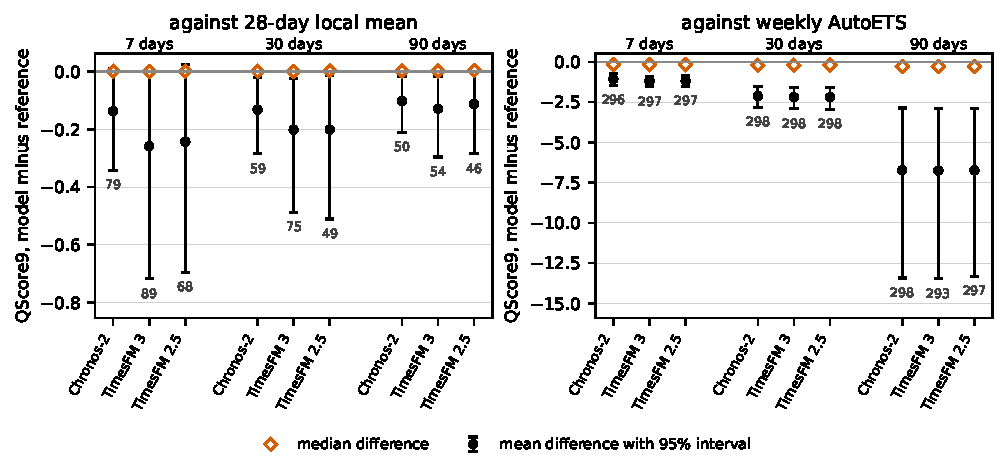
\includegraphics[width=\textwidth]{fig-paired-differences}
\caption{The 18 declared comparisons. Filled circles: mean difference (model minus reference \qs{}) with its
pointwise 95 percent repository-bootstrap interval. Open diamonds: median difference. The number under each
interval is the count of repositories, of 300, where the model's score is lower. Note the different vertical
scales.}
\label{fig:paired}
\end{figure}

\paragraph{Against the local mean.} In all nine cells the mean difference is negative, favoring the model,
from $-0.101$ (Chronos-2, 90 days) to $-0.258$ (TimesFM 3, 7 days), and the bootstrap interval excludes
zero in five cells: the three 30-day cells and the 90-day cells of Chronos-2 and TimesFM 3. The three 7-day
intervals and TimesFM 2.5 at 90 days include zero. In all nine cells the median difference is positive,
favoring the reference, and the model's score is lower on only 46 to 89 of the 300 repositories. The
signed-rank test rejects in all nine cells after adjustment (largest adjusted $p$ 0.0067, TimesFM 3 at 7
days); because every median is positive, the location shift the test detects favors the reference. The
signed-rank test is not a test of the mean, and the bootstrap interval is pointwise, not simultaneous; the
two statements do not contradict each other. The mean is carried by a minority of repositories with large
gains: in the declared scale review the five largest positive repository gains account for 88.5 to 94.3
percent of all positive gain against the local mean, and the leave-one-repository-out mean gain stays
positive in every cell (Appendix Table~\ref{tab:scale}). Ratio skill against the local mean is defined for
only 209, 239 and 259 of 300 repositories at 7, 30 and 90 days, because the reference's loss is zero on the
others; the report does not headline a ratio.

\paragraph{Against AutoETS.} In all nine cells both the mean and the median difference are negative, the
model's score is lower on 293 to 298 of 300 repositories, and the signed-rank test rejects in all nine; both
summaries favor the model. Mean differences grow with horizon, from $-1.07$ to $-1.19$ at 7 days to $-6.72$
to $-6.75$ at 90 days, and the 90-day intervals are wide. The reason is in the reference: AutoETS's nominal
80 percent intervals cover 98.6 to 98.8 percent of target days pooled over the panel (a declared secondary
summary), and in a width diagnostic requested after the run within that declared analysis its median 90-day
daily interval width is 0.79 stars per day in the smallest stratum, 3.60 in the middle one and 49.69 in the
top one (Appendix Table~\ref{tab:autoets}). Six fits at each horizon, from two repositories, selected
multiplicative seasonality, all in the top stratum; the specification counts were also requested after the
run. AutoETS is a weak uncertainty reference on this panel.

\paragraph{By stratum and calibration.} Pooled \qs{} by stratum (Appendix Table~\ref{tab:stratum}) holds
stratum means only: in the top stratum the three models' pooled scores are below the local mean's at every
horizon; in the smallest stratum the local mean's is below all three at every horizon; in the middle stratum
the four differ by less than 0.012 at every horizon; and AutoETS is far above all of them at every scale. The
typical repository by stratum is not in the declared tables. A post-hoc reading of the saved per-repository
accounting file, which adds no test, gives it: the median difference against the local mean is positive,
favoring the reference, in every stratum and every cell, and the models score lower on 5 to 18 of 100
repositories in the smallest stratum, 10 to 34 in the middle one and 26 to 38 in the top one. So the stratum
means and the typical repository disagree within the top stratum as the panel mean and the typical repository
disagree overall. Inclusive 80 percent coverage of the repaired deciles over the panel is 0.824 to 0.837 for
Chronos-2, 0.880 to 0.910 for TimesFM 3, 0.906 to 0.924 for TimesFM 2.5, 0.941 to 0.955 for the local mean
and 0.986 to 0.988 for AutoETS (Appendix Table~\ref{tab:calibration}). On discrete counts a correct quantile
can overcover \citep{czado2009}, so these are descriptive.


\section{Post-hoc accounting of the saved run}

This section is post-hoc. It was computed on 2026-09-14 from the saved forecasts after the registered
results were seen, adds no test, and does not change the status of anything above. Each window's \qs{} is
split exactly into three parts, each divided by the full horizon: the loss on zero-target days, which for
nonnegative quantiles is $\frac{2}{9h}\sum_{y_t = 0}\sum_\tau (1-\tau) q_{t,\tau}$; the loss on positive days
from quantiles above the target (overprediction); and the loss on positive days from quantiles below it
(underprediction). The parts sum to \qs{} on all 48,600 rows to floating-point tolerance, and the same
within-repository and across-repository averaging reproduces the 18 registered mean differences. The
decomposition locates where a loss difference arises; it says nothing about why a model forecast what it did.

\begin{table}[t]
\centering\small
\caption{Post-hoc. The mean difference against \lm{} and its three parts, model minus reference; negative
favors the model. The parts sum to the total.}
\label{tab:posthoc}
\begin{tabular}{llrrrr}
\toprule
Model & $h$ & Total & Zero days & Positive, overprediction & Positive, underprediction \\
\midrule
Chronos-2 & 7 & -0.137 & 0.005 & -0.095 & -0.048 \\
Chronos-2 & 30 & -0.132 & 0.005 & -0.156 & 0.019 \\
Chronos-2 & 90 & -0.101 & 0.004 & -0.184 & 0.078 \\
TimesFM 3 & 7 & -0.258 & 0.004 & -0.091 & -0.171 \\
TimesFM 3 & 30 & -0.201 & 0.006 & -0.150 & -0.057 \\
TimesFM 3 & 90 & -0.128 & 0.011 & -0.187 & 0.047 \\
TimesFM 2.5 & 7 & -0.243 & 0.012 & -0.088 & -0.167 \\
TimesFM 2.5 & 30 & -0.201 & 0.014 & -0.163 & -0.052 \\
TimesFM 2.5 & 90 & -0.112 & 0.015 & -0.209 & 0.082 \\
\bottomrule
\end{tabular}
\end{table}

Table~\ref{tab:posthoc} gives the parts for the nine cells against the local mean. The finding in one
sentence: the mean gain sits on positive days where the local mean overpredicts, and the zero-day part is
small beside it. The zero-day part is positive, against the models, in every cell, from 0.004 to 0.015: small
beside mean differences of $-0.101$ to $-0.258$, but in every cell larger than that cell's median
difference in Table~\ref{tab:lm}, where the medians run from 0.0003 to 0.0041. The overprediction part favors the models in every cell,
from $-0.088$ to $-0.209$. The underprediction part favors the models at 7 days, where for both TimesFM
models it is the larger of the two positive-day parts, and favors the local mean at 90 days, where the
models' underprediction loss exceeds the local mean's. Why the local mean overpredicts on those days is not
something the accounting tests.

\begin{figure}[t]
\centering
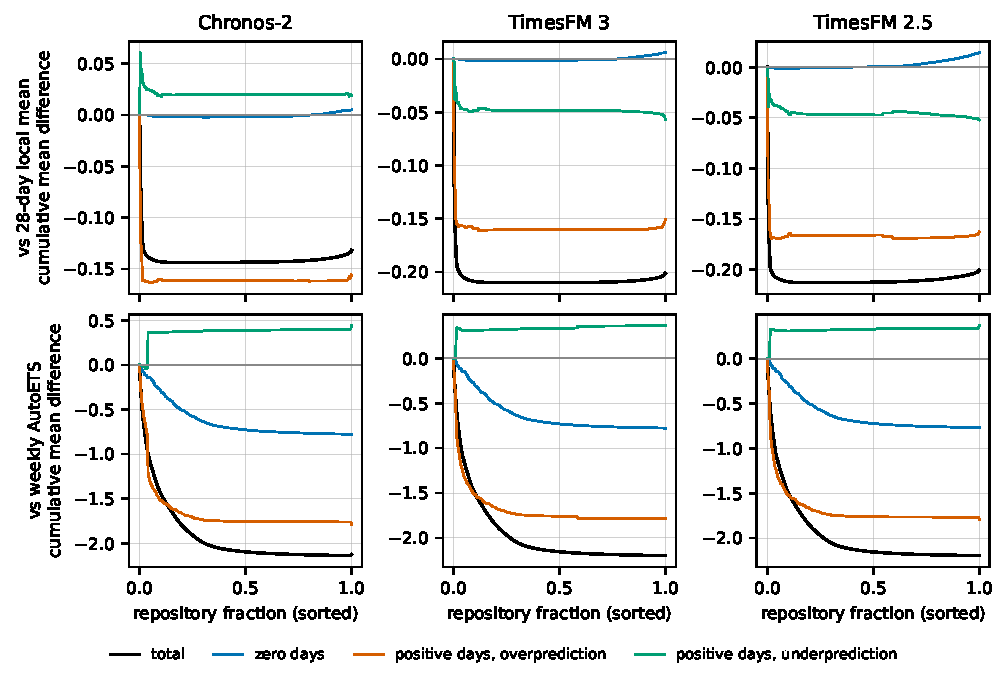
\includegraphics[width=\textwidth]{fig-posthoc-cumulative-h30}
\caption{Post-hoc. Signed cumulative contribution to the mean difference at horizon 30, repositories sorted
by their total difference (ascending) and the cumulative sum divided by 300, so each curve ends at its mean.
Top row: against \lm{}; bottom row: against \aets{}. Vertical scales differ between rows.}
\label{fig:cumulative}
\end{figure}

Figure~\ref{fig:cumulative} shows the same accounting as cumulative curves. Against the local mean, the total
drops to its final level within the first few percent of repositories and then drifts slightly upward over
the remaining majority, which lose by small amounts; against AutoETS the gain accrues across most of the
panel, and its largest part is overprediction on positive days, with a zero-day part between $-0.768$ and
$-0.777$. Appendix Figure~\ref{fig:zerofraction} places each repository by its context zero fraction: against
the local mean the large model gains are at low zero fractions and the small model losses cluster at high
ones, while against AutoETS nearly every repository at every zero fraction favors the model.


% Study 2, the question. Input from paper.tex; every number traces to sources.md and is asserted by
% check_numbers.py. Macros are provided in case the file is compiled before paper.tex defines them.
\providecommand{\lm}{\texttt{local\_mean\_28}}
\providecommand{\qs}{QScore9}
\providecommand{\hc}{\texttt{hurdle\_count\_28}}

\section{Study 2: the question}
\label{sec:s2question}

Study 2 was registered on 2026-09-14 as a dated addition to the protocol, at commit
\texttt{df55867c982dfe2bb6e1152ec8ae93e3cd228c45} (full protocol SHA-256 at registration
\texttt{33cefd8e34fea973e6747d1ba3fe565051e215c5d1b7f6553b266c1be7a66360}), after Study 1's results were
seen, to be tested on data declared separately from Study 1's. It asks two questions about a frozen foundation
model's forecast of a daily count. First, whether replacing the model's own probability of a zero day with a
context-only occurrence probability, while keeping the model's completed positive conditional distribution,
lowers \qs{}. Second, whether that positive component, the model's own law for the size of a positive day,
improves on a fixed count hurdle whose positive law is a shifted Poisson fitted to the last 28 context days.
The registered text allows that a lower loss on zero days may coexist with a higher loss on positive days,
and says that the net sign, the typical-series sign and a null outcome are all reportable. The registration
named three external domains; the dated addition of 2026-10-12, decided before any target value was opened,
deferred NYC 311 requests and Wikipedia pageviews, and the registered October holdout lapsed, so the
occurrence test ran on one external domain, npm package downloads, and on the registered synthetic grid
(Section~\ref{sec:notrun}). Nothing in Study 2 amends Study 1's sample, forecasts, scores, comparisons or
conclusions; the completion of a model's deciles into a count distribution is a Study 2 assumption and is
not attributed to Study 1.

The question follows from the Study 1 accounting of Section~\ref{sec:results} and the post-hoc parts of
Table~\ref{tab:posthoc}. A daily count forecast has two parts, whether anything happens and how much
happens when it does, and the foundation models supply neither part on its own terms: their native output
is nine quantiles of a continuous forecast, clipped at zero, and a zero day enters the score only through
whichever deciles the model placed at or below zero. In Study 1 the models' mean gain against \lm{} sat on
positive days where the local mean overpredicts, while the zero-day part of the paired difference was
positive, against the models, in every cell, from 0.004 to 0.015, in every cell larger than that cell's
median difference, which ran from 0.0003 to 0.0041; the typical repository favored the local mean, with the
models lower on only 46 to 89 of 300 repositories. A reading made after those results, and registered as a
separate study rather than tested on Study 1's run, is that the models' size forecasts carry the gain and
their occurrence forecasts carry the loss, so that an occurrence probability estimated from the context
alone, substituted for the model's zero mass, would lower the loss where the models lose and keep it where
they win. Whether the substitution helps is the question, not the premise.

\paragraph{Four forecasters, three of them run.} The two contrasts compare forecasters that differ in
where the occurrence probability and the positive law come from. The \emph{completed} control takes both
from the model. The \emph{hurdle} variant takes the occurrence from the context, the 28-day Jeffreys
estimate, and the positive law from the model. The count hurdles take both from the context: the same
occurrence estimate with a shifted-Poisson positive law (\hc{}, the registered comparator) or with the
empirical distribution of the positive context values (\texttt{hurdle\_empirical\_28}, declared secondary).
The first contrast changes the occurrence alone; the second changes the positive law alone. The fourth cell
of that two-by-two, the model's own occurrence with a count positive law, was not registered and is not
computed in this paper; Section~\ref{sec:discussion} says what it would separate. The registered
\texttt{dynamic\_count} baseline has its own occurrence estimate and its own positive law and sits outside
the two-by-two.

\paragraph{What is known.} A literature re-check for work since 2026-09-13, run on 2026-10-12 and recorded
in the repository, and a wider sweep of 2026-10-16, set what this paper may claim. The construction is not new
in its parts. Frozen foundation models have been evaluated on sparse daily counts as an event-ranking task
without a proper score \citep{schoess2026}, and on daily counts under calibration measures with the sparse
series binned away \citep{adler2025}; an occurrence-times-size hurdle has been applied to frozen Chronos-2
output on monthly spare-parts demand, judged by point and service measures, where it trailed plain
re-centring \citep{chin2026}; and TimesFM 3's nine-decile pinball loss on simulated intermittent counts has
been reported as no better than the history's empirical deciles, in a study whose protocol was pre-registered
and self-archived before any forecast was produced \citep{ebrahim2026, ebrahim2026zenodo}, the nearest
precedent to this paper's registration, a simulation with no third-party timestamp before its runs. That
aggregate and per-series rankings of zero-shot models can disagree has been shown on a marketplace panel and
on M5 with medians, win counts and a weighting sensitivity beside the means \citep{islam2026}, on
quick-commerce demand \citep{kim2026}, on financial series where the pooled loss sat in a few assets
\citep{brini2026} and by trend strength \citep{cherif2026}; the mean scaled score has been recommended in
print over medians, ranks and win rates on intermittent data \citep{corani2026}. A later test window on
familiar entities does not establish generalization to unseen ones \citep{moghadasi2026}, later windows of
known series leak through temporal dependence \citep{qiao2026}, and pre-training contamination of frozen
forecasters is now audited directly \citep{li2026}. Daily GitHub stars are a live-benchmark target: on the
400 most-starred repositories, under a scaled CRPS aggregated by the median series, the foundation models
hold the top ranks and the typical series favors them \citep{garza2026}, where on the population sample of
Study 1 the typical repository favors the local mean; a second live benchmark finds static rankings of the
same model families inverting under live evaluation \citep{wen2026}. Earlier items in the protocol's lineage
bear on the same ground \citep{tsantilis2025, zodiac2026, fevbench2026, meyer2025}; hurdle-count forecasting
without foundation models has current reference points \citep{damato2026, bai2026}, and one zero-shot model
built for frequent zeros was released in the window with a quantile head and no count head
\citep{exaone2026}.

What neither search found, as of 2026-10-12 and again as of 2026-10-16, is a published evaluation in which a
context-only occurrence probability replaces the zero mass of frozen Chronos-2 or TimesFM forecasts while
their completed positive conditional distribution is kept, judged by a proper quantile score against a
completed-unwrapped control and matched count hurdles on sparse daily counts; nor a registered protocol
fixed before access to real data, with a public audit and redesign of a first version, for any
foundation-model forecasting evaluation. ``Not found'' means those searches did not find it, not that it
does not exist; two routes failed and papers under review are not visible by any route used. The claim the
paper makes, stated in full in Section~\ref{sec:discussion}, is the registered combination on daily npm
download counts and the registered synthetic grid, with Study 1's GitHub star counts entering through the
raw comparison alone, and nothing broader.


% Study 2, the registered design as it stands after the dated additions of 2026-10-12, 2026-10-15 and
% 2026-10-16. Input from paper.tex; every number traces to sources.md and is asserted by check_numbers.py.
% The frame, completion, baseline and family detail is in study2-design-detail.tex (Appendix E). Macros are
% provided in case the file is compiled before paper.tex defines them.
\providecommand{\lm}{\texttt{local\_mean\_28}}
\providecommand{\aets}{\texttt{autoets\_weekly}}
\providecommand{\qs}{QScore9}
\providecommand{\hc}{\texttt{hurdle\_count\_28}}

\section{Study 2: the registered design}
\label{sec:s2design}

What follows is the design as registered on 2026-09-14 at commit \texttt{df55867}, as it stands after the three
dated additions that bear on it: the addition of 2026-10-12, committed at \texttt{8db0d73}, which
records the lapses of September 2026 and fixes the families of this paper; the addition of 2026-10-15,
committed at \texttt{5be2ce9}, which fixes the availability rule for one secondary score, both decided
before any Study 2 target value was accessed; and the addition of 2026-10-16, committed at \texttt{1c09ac8},
made after the npm scores were seen, which changes nothing in the design and records how three zero days
served by the source are handled (Section~\ref{sec:s2results}). Nothing above any addition's heading
changed, and the registered bytes remain byte prefixes of the protocol file. The frame and sampling rule,
the completion, the baselines, the family tables, the secondary scores, the seeds and the gate are in
Appendix~\ref{app:s2design}.

\paragraph{Domains and panels.} The registration names three external domain slots: package downloads,
with npm as the primary source and PyPI through ClickPy as its sole operational fallback; NYC 311 requests;
and English Wikipedia pageviews. Each slot aims at 300 series, 100 in each of three context-zero-fraction
strata, $[0, 0.5)$, $[0.5, 0.9)$ and $[0.9, 1]$, computed on the last 90 context days, which the protocol
calls a balanced stress-test panel, not an estimate of a platform's natural prevalence of sparsity. Series
are drawn by hash from a frozen frame with no popularity filter; a stratum with fewer than 100 complete
candidates keeps what it has, with no transfer of slots. The addition of 2026-10-12 defers NYC 311 and
Wikipedia, so this paper's external component is the packages domain alone (Section~\ref{sec:s2panel}).

\paragraph{Calendar.} The retrospective calendar has context start $A$ = 2025-09-01, common endpoint $E$ =
2026-08-31 and $K = 3$ cutoffs at $c_j = E - (30j - 1)$ days for $j = 3, 2, 1$: 2026-06-03, 2026-07-03 and
2026-08-02, with 275, 305 and 335 context days. Context stops the day before the cutoff; the target block
runs from the cutoff for 7 or 30 days, so the three 30-day blocks partition the trailing 90 days and do not
overlap, and the 7-day blocks share the same origins. Selection strata are computed on $c_1 - 90$ through
$c_1 - 1$, 2026-03-05 through 2026-06-02, and frozen for all origins. Package day labels are UTC. No model
sees another series or any covariate, and no horizon is counted as an independent entity.

\paragraph{Models and variants.} The three foundation models are the Study 1 pins: \texttt{amazon/chronos-2}
at \texttt{29ec3766d36d6f73f0696f85560a422f50e8498c}, \texttt{google/timesfm-3.0-pytorch} at
\texttt{43046b85ec22d584a13f8098c2ed39c889e129c2} and \texttt{google/timesfm-2.5-200m-pytorch} at
\texttt{1d952420fba87f3c6dee4f240de0f1a0fbc790e3}, pinned on 2026-09-12 and run univariate at batch size one
on one GPU. For each model and origin one base forecast is saved and three variants are scored from it, with
no refitting: \emph{raw}, the nine native deciles after Study 1's clipping and crossing repair; \emph{completed},
the count distribution $F$ obtained from those deciles by a fixed completion (linear interpolation through
the origin and the nine knots, an exponential upper tail with a finite first moment, half-up rounding to a
count), which is the control; and \emph{hurdle}, the same completed law with its zero mass replaced by the
28-day Jeffreys occurrence estimate $p$, so that $H(0) = 1 - p$ and $H(k) = 1 - p + p\, G_+(k)$ with $G_+$
the model's own positive conditional law $[F(k) - F(0)] / [1 - F(0)]$. The hurdle and completed variants
differ in nothing else. $G_+$ is the completed marginal law truncated at one, not a separately produced size
forecast; Section~\ref{sec:discussion} returns to this.

\paragraph{Baselines and comparators.} Seven baselines are scored at every origin: \lm{} and \aets{} from
Study 1, a negative-binomial local level, a Poisson, the two count hurdles and the dynamic count. The two
count hurdles share the foundation-model hurdle's occurrence rule and differ from it in the positive law
alone: \hc{} fits $1 + \text{Poisson}(\lambda)$ to the positive days of the last 28, and
\texttt{hurdle\_empirical\_28}, declared secondary, uses the empirical distribution of those values. The
dynamic count, \texttt{dynamic\_count}, has its own discounted occurrence estimate and its own
negative-binomial positive law. None of the three has a positive law from a foundation model.

\paragraph{The confirmatory families.} The registration declared one external family of 54 tests, for each
of three domains, three models and two horizons the hurdle against its own completed control, the hurdle
against \hc{}, and the raw deciles against \lm{}, that is $3 \times 3 \times 2 \times 3 = 54$. The addition
of 2026-10-12 fixes this paper's external family as the eighteen packages-domain tests E01 to E18, exactly as
registered and listed in Appendix Table~\ref{tab:s2family}, with one Benjamini-Hochberg adjustment at
$q = 0.05$ over those eighteen; E19 to E54 form, when NYC 311 and Wikipedia are run, one family of 36 with
its own single correction. The settings are Study 1's: the paired difference is model minus reference, so
negative favors the model; the mean carries a pointwise 95 percent percentile interval from 20,000 bootstrap
replicates of whole series (bootstrap seed 20260917); a two-sided approximate Wilcoxon signed-rank test on
series averages omits zero differences; medians, wins, ties and losses are reported; inference is
conditional on the fixed dates. The synthetic family is six tests at horizon 30, S01 to S06 (Appendix
Table~\ref{tab:s2synfamily}): each model's hurdle against its own completed control and against \hc{},
pooling all 18 cells with equal cell weight, one adjustment at $q = 0.05$. Every other contrast, the strata,
the scaled score, the Brier score, the CRPS, the PIT and the accounting parts, is secondary and adds no
test. Because both families pool their entities with equal weight, 209 series on an unscaled score and 18
cells, each confirmatory answer speaks for whatever dominates its pool; Section~\ref{sec:s2results} reads
the declared strata beside them.

\paragraph{The synthetic grid.} With $\pi = 1 - z$, the occurrence indicator $Z_t$ is a stationary Markov
Bernoulli chain with $P(Z_t = 1 \mid Z_{t-1} = a) = \pi + \rho\,(a - \pi)$; independently $X_t \sim
\text{Poisson}(\mu_{+} - 1)$ and $Y_t = Z_t (1 + X_t)$, so the generator's positive law is the count
hurdle's own family. The grid is the full product of $z \in \{0.2, 0.8, 0.95\}$, $\mu_{+} \in \{1, 5, 25\}$
and $\rho \in \{0, 0.8\}$: 18 cells, each with 30 independent replicates of 270 observations, the first
context 180 days, origins at indices 180, 210 and 240, horizons 7 and 30, so 540 series in all, with the
synthetic root seed 20260918. The same models, completion, baselines and scores apply; an oracle that knows
the generator parameters and the last observed state is a diagnostic, not a competitor. Origins are averaged
within each replicate and cell, then cells within replicate; the paired test and the bootstrap use the 30
replicate blocks. Seven-day scores and individual cells are secondary, and no cell or generator was chosen
because it reproduces Study 1.


% Study 2, the achieved npm panel, from the committed panel files and the status file. Input from main.tex
% in the extension; every number traces to sources.md and is asserted by check_numbers.py. Macros are
% provided in case the file is compiled before main.tex defines them.
\providecommand{\qs}{QScore9}

\section{Study 2: the achieved npm panel}
\label{sec:s2panel}

The packages domain is npm. Its panel was frozen on 2026-10-15 01:57 UTC and verified at 02:00 UTC, inside
the reset readiness deadline of 2026-10-20 23:59 UTC, so the registered PyPI substitution was not invoked.
Everything in this section is computed from the context window alone, 2025-09-01 to 2026-06-02; as of
2026-10-15, a statement to be re-checked on the posting day against the same status file, no target value
of 2026-06-03 to 2026-08-31 had been opened.

\paragraph{Inventory and candidate walk.} The frozen inventory is the registry's replication feed read in
4,493 pages of at most 1,000 names between 2026-10-14 00:23 and 02:04 UTC: 4,486,927 package names, scopes
included. The walk visited the first 12,943 names in candidate-hash order and requested each one's registry
document: 10,000 were eligible, created before 2025-09-01; 2,918 were ineligible on their creation time or
frame; and 25 were excluded because the registry answered HTTP 404 for the name. The walk stopped when the
pool was full. Because it did not exhaust the inventory, the size of the eligible frame is estimated from
the visited prefix, as the inventory size times the eligible share of the visited names: about 3,466,682
packages, with exact bounds of 10,000 and 4,483,984. The candidate-pool inclusion probability of an eligible
package is correspondingly about 0.0029, with bounds 0.0022 and 1. These are estimates from a hash-ordered
prefix, not counts.

\paragraph{The context pull and the strata.} The 10,000 candidates' daily download counts from 2025-09-01 to
2026-06-02 were requested from the download-counts API; 9,998 answered completely and 2 were excluded
because the API answered HTTP 404 for the package (\texttt{@zitterorg/modi-quaerat-voluptas},
\texttt{walk-logger}), the only context-stage exclusions. Of the 12,762 attempts to that host, 9,998 returned
the range, 40 returned 404, 2,708 returned 429, 2 returned 504 and 14 timed out; every refusal was retried
later from the saved captures without excluding a candidate. On the stratum window of 2026-03-05 to
2026-06-02 the 9,998 complete candidates fell 2,431 in the dense stratum (zero fraction below 0.5), 7,558 in
the sparse stratum (0.5 to below 0.9) and 9 in the very sparse stratum (0.9 and above). The achieved panel
is therefore 209 series: 100 dense, 100 sparse and 9 very sparse, the first in selection-hash order within
each stratum, with 91 very-sparse slots unfilled (Table~\ref{tab:s2panel}). The 209 names were created
between 2011-08-26 and 2025-08-08; 80 of them are scoped names.

\begin{table}[t]
\centering\small
\caption{The achieved npm panel by context-zero-fraction stratum, computed on 2026-03-05 to 2026-06-02:
the complete candidates among the 9,998 of the frozen pool, the series taken and the unfilled slots. The
stratum bounds are the registered $[0, 0.5)$, $[0.5, 0.9)$ and $[0.9, 1]$.}
\label{tab:s2panel}
\begin{tabular}{llrrr}
\toprule
Stratum & Zero fraction & Complete candidates & Taken & Unfilled \\
\midrule
dense & $[0, 0.5)$ & 2,431 & 100 & 0 \\
sparse & $[0.5, 0.9)$ & 7,558 & 100 & 0 \\
very sparse & $[0.9, 1]$ & 9 & 9 & 91 \\
\bottomrule
\end{tabular}
\end{table}

\paragraph{Why the third stratum is short.} The registered rule fixes the candidate pool at the first
10,000 eligible names in hash order and forbids a larger pool, a transfer of unused slots and any
alternative filter, so the stratum holds every complete candidate that qualified and no more. Only 9 of
9,998 complete candidates had zero downloads on at least 90 percent of the 90 stratum days. A reading, not a
measured fact: npm counts every tarball request, including mirrors and automated clients, so a published
package is rarely without a download for most of a quarter, and the very sparse stratum that is natural for
GitHub stars is close to empty for npm downloads. The stratum is reported as achieved; the confirmatory
family pools all 209 series as registered, strata being secondary descriptors, and any per-stratum table
shows $n = 9$ for the very sparse stratum.

\paragraph{The pull's budget and the API's limits.} The approval was 36,000 requests and 13 hours,
cumulative over the inventory, the walk and the context pull. The pull used 30,198 HTTP attempts: 12,943 to
the registry host, 12,762 to the download-counts host and 4,493 to the replication host, over 52
invocations totalling 45,508 seconds (12 hours and 38 minutes), from 2026-10-14 00:23 UTC to 2026-10-15 01:57
UTC. Attempts were spaced at least one second apart, and at least three seconds from 2026-10-14 22:51 UTC,
when the download API was answering about 20 requests a minute. The download API returned 429 to 2,708
attempts; three in a row for one key stopped the invocation, which resumed later from the saved captures.
From 2026-10-14 08:44 UTC the download API timed out or answered 504 until at least 10:25 UTC and answered
again at 21:37 UTC; each such stop wrote nothing and excluded no candidate. No documented request quota for
the download-counts API was found in the governing documents, and 30,198 attempts in about 26 hours is far
below the one stated line, five million requests a month; the redistribution review records the 429 answers
as the pull repeatedly reaching npm's throttle and honouring it.

\paragraph{One series at 7.6 million downloads a day.} The dense stratum holds the package
\texttt{aggregate-error}, whose last 28 context days before the first cutoff average 7,637,136 downloads a
day; the next largest last-28 mean in the panel is about 13,000. Equal series weights, as registered, mean
that the mean paired difference of the unscaled \qs{} over 209 series is that one series' difference divided
by 209 plus a remainder from the other 208, whose losses are of a different order; the series-bootstrap
interval inherits the same dependence. The median difference, the win count and the signed-rank test are
rank-based and unaffected; the scaled \qs{}, which divides each window's loss by the context mean, is
secondary. The paper states this when it reports the mean, and this is a property of the registered design,
not a defect found in it. The same series is the case behind the availability rule of 2026-10-15
(Section~\ref{sec:s2design}): no discrete CRPS can be certified for it within the registered work limit, so
its CRPS is recorded as unavailable and counted in the denominators.

\paragraph{Data statement.} The daily counts of the 209 series were obtained from the npm download-counts
API, \url{https://api.npmjs.org/downloads/range}, between 2026-10-14 and 2026-10-15 UTC, for 2025-09-01 to
2026-06-02; the targets for 2026-06-03 to 2026-08-31 are to be obtained under a separate target-access
approval. Package names and creation timestamps come from the npm public registry,
\url{https://registry.npmjs.org}, and from its replication feed, \url{https://replicate.npmjs.com}. A
download is a tarball request as npm counts it, including mirrors, build servers and automated clients, and
is a directional indicator rather than a count of users. npm, Inc.\ states no licence for the download
counts, and its Open-Source Terms of 2022-03-10, read as governing the public registry and its public APIs,
contain no restriction on their redistribution; replication of registry data through the public
APIs is expressly allowed. Names are as the registry served them at acquisition and may since have been
removed. The pull reached npm's rate limit 2,708 times and honoured it. The project's compilation of the
selection, the derived fields and the documentation is released under CC BY 4.0; no licence is asserted over
the counts as such. Maintainer names, e-mail addresses, descriptions and raw registry documents are not
published. The manifest and selection files are in the repository; the aggregated daily counts are
published with the paper. npm is a registered trademark of npm, Inc.; no npm logo is used.


% Study 2, the results, from the inference, integrity and post-hoc files of the two runs under reports/ and
% the post-hoc dynamic-occurrence directory. Input from paper.tex; every number traces to sources.md and is
% asserted by check_numbers.py. Macros are provided in case the file is compiled before paper.tex defines
% them.
\providecommand{\lm}{\texttt{local\_mean\_28}}
\providecommand{\aets}{\texttt{autoets\_weekly}}
\providecommand{\qs}{QScore9}
\providecommand{\hc}{\texttt{hurdle\_count\_28}}

\section{Study 2: results}
\label{sec:s2results}

Tables~\ref{tab:s2ext} and~\ref{tab:s2syn} give the eighteen external and the six synthetic comparisons
with the columns of Tables~\ref{tab:lm} and~\ref{tab:ae}; differences are model variant minus reference, so
negative favors the variant, and every external mean is carried by one series (Section~\ref{sec:s2panel}).
Twelve of the eighteen external tests and five of the six synthetic tests reject at $q = 0.05$ after one
adjustment per family; of the twelve, ten reject for the model variant and two against it, and all five
synthetic rejections are against the hurdle variant. Figure~\ref{fig:s2npm} shows the 209 paired differences
behind each external row. Each run ran once on 2026-10-15 with no failed window, and every one of the 20,064
npm and 55,080 synthetic scores was recomputed from the saved forecasts with no disagreement
(Appendix~\ref{app:s2repro}).

\begin{table}[t]
\centering\footnotesize\setlength{\tabcolsep}{3.5pt}
\caption{The eighteen declared external comparisons on the npm panel. Differences are model variant minus
reference \qs{}, averaged over three origins within series and then over 209 series; negative favors the
variant. The contrast names the pair: the model's hurdle against its completed control, the hurdle against
\hc{}, or the raw deciles against \lm{} (the full tuples are in Appendix Table~\ref{tab:s2family}). The
interval is the pointwise 95 percent percentile interval from 20,000 series-cluster bootstrap replicates.
``Lower / tied / higher'' counts the series (of 209) where the variant's score is below, equal to or above
the reference's. $p$ is the Benjamini-Hochberg adjusted two-sided Wilcoxon signed-rank $p$-value over the
18 tests. Every mean in this table is carried by the series \texttt{aggregate-error}
(Section~\ref{sec:s2panel}); the medians, counts and tests are rank-based and describe the typical series.}
\label{tab:s2ext}
\begin{tabular}{lllrrcrcl}
\toprule
ID & Model & Contrast & $h$ & Mean & 95\% interval & Median & Lower / tied / higher & Adjusted $p$ \\
\midrule
E01 & Chronos-2 & hurdle vs completed & 7 & 152 & [0.1846, 455.2] & -0.01376 & 121 / 2 / 86 & 0.203 \\
E02 & Chronos-2 & hurdle vs count hurdle & 7 & -5,090 & [-15,175, -31.08] & -0.01587 & 129 / 12 / 68 & $3.72 \times 10^{-11}$ \\
E03 & Chronos-2 & raw vs local mean & 7 & -2,884 & [-8,601, -17.33] & 0.007856 & 92 / 0 / 117 & 0.596 \\
E04 & Chronos-2 & hurdle vs completed & 30 & 90.24 & [0.2273, 269.7] & -0.0002469 & 105 / 2 / 102 & 0.449 \\
E05 & Chronos-2 & hurdle vs count hurdle & 30 & -6,563 & [-19,596, -30.03] & -0.06173 & 150 / 9 / 50 & $7.06 \times 10^{-21}$ \\
E06 & Chronos-2 & raw vs local mean & 30 & -4,734 & [-14,149, -15.84] & -0.002372 & 112 / 0 / 97 & 0.0119 \\
E07 & TimesFM 3 & hurdle vs completed & 7 & 176.9 & [0.2669, 529.4] & 0.001058 & 94 / 8 / 107 & 0.236 \\
E08 & TimesFM 3 & hurdle vs count hurdle & 7 & -5,416 & [-16,153, -31.67] & -0.007407 & 116 / 18 / 75 & $3.61 \times 10^{-8}$ \\
E09 & TimesFM 3 & raw vs local mean & 7 & -3,235 & [-9,650, -18.24] & -0.002297 & 112 / 1 / 96 & 0.0438 \\
E10 & TimesFM 3 & hurdle vs completed & 30 & 128.5 & [0.5058, 383.8] & 0.00321 & 81 / 8 / 120 & 0.00215 \\
E11 & TimesFM 3 & hurdle vs count hurdle & 30 & -6,792 & [-20,280, -31.3] & -0.0716 & 161 / 17 / 31 & $3.19 \times 10^{-25}$ \\
E12 & TimesFM 3 & raw vs local mean & 30 & -5,001 & [-14,947, -16.86] & -0.005016 & 125 / 1 / 83 & $3.82 \times 10^{-5}$ \\
E13 & TimesFM 2.5 & hurdle vs completed & 7 & 253.9 & [0.5046, 759.9] & -0.002116 & 109 / 3 / 97 & 0.628 \\
E14 & TimesFM 2.5 & hurdle vs count hurdle & 7 & -5,847 & [-17,446, -30.83] & -0.006349 & 115 / 7 / 87 & $2.66 \times 10^{-5}$ \\
E15 & TimesFM 2.5 & raw vs local mean & 7 & -3,743 & [-11,179, -17.41] & 0.01696 & 84 / 1 / 124 & 0.746 \\
E16 & TimesFM 2.5 & hurdle vs completed & 30 & 110.3 & [0.6883, 328.7] & 0.0009877 & 101 / 1 / 107 & 0.0276 \\
E17 & TimesFM 2.5 & hurdle vs count hurdle & 30 & -6,918 & [-20,665, -29.9] & -0.06938 & 160 / 9 / 40 & $1.77 \times 10^{-23}$ \\
E18 & TimesFM 2.5 & raw vs local mean & 30 & -5,109 & [-15,279, -15.49] & -0.003695 & 113 / 1 / 95 & 0.00204 \\
\bottomrule
\end{tabular}
\end{table}

\begin{table}[t]
\centering\footnotesize\setlength{\tabcolsep}{3.5pt}
\caption{The six declared synthetic comparisons at horizon 30. Differences are model variant minus reference
\qs{}, averaged over three origins within each replicate and cell, then over the 18 cells with equal weight,
so that each of the 30 replicate blocks carries one paired difference; negative favors the variant. The
interval is the pointwise 95 percent percentile interval from 20,000 replicate-block bootstrap replicates.
``Lower / tied / higher'' counts the blocks (of 30) where the variant's score is below, equal to or above
the reference's. $p$ is the Benjamini-Hochberg adjusted two-sided Wilcoxon signed-rank $p$-value over the
6 tests.}
\label{tab:s2syn}
\begin{tabular}{lllrrcrcl}
\toprule
ID & Model & Contrast & $h$ & Mean & 95\% interval & Median & Lower / tied / higher & Adjusted $p$ \\
\midrule
S01 & Chronos-2 & hurdle vs completed & 30 & 0.08599 & [0.03836, 0.1401] & 0.05554 & 6 / 0 / 24 & 0.00415 \\
S02 & Chronos-2 & hurdle vs count hurdle & 30 & 0.05211 & [0.01686, 0.09227] & 0.04737 & 9 / 0 / 21 & 0.0111 \\
S03 & TimesFM 3 & hurdle vs completed & 30 & 0.08662 & [0.03837, 0.1429] & 0.06144 & 6 / 0 / 24 & 0.00676 \\
S04 & TimesFM 3 & hurdle vs count hurdle & 30 & 0.0215 & [-0.006569, 0.04947] & 0.03119 & 11 / 0 / 19 & 0.12 \\
S05 & TimesFM 2.5 & hurdle vs completed & 30 & 0.08769 & [0.04316, 0.1382] & 0.06743 & 5 / 0 / 25 & 0.00415 \\
S06 & TimesFM 2.5 & hurdle vs count hurdle & 30 & 0.06109 & [0.02299, 0.09881] & 0.06027 & 9 / 0 / 21 & 0.00798 \\
\bottomrule
\end{tabular}
\end{table}

\paragraph{Three zero days in the npm targets.} After the run was scored, the saved targets were found to
read 0 for every one of the 209 series on 2026-07-12 and 2026-08-14, and 0 for \texttt{aggregate-error}
alone on 2026-06-25, between days of millions (Appendix~\ref{app:s2tables}). The registered completeness
rule, fixed before any target was seen, does not test for a source-wide zero, so the three days were scored
as served; each falls in one horizon-30 block and in no horizon-7 block. npm's own records report no outage
or backfill for them, and a public thread records two earlier episodes in which whole days read 0 for nearly
every package and were later restored \citep{npm-community-150808}. The dated addition of 2026-10-16 to the
protocol, item 6, made after the scores were seen, keeps the registered analysis of the data as served as
the confirmatory result for E01 to E18 and asks that a post-hoc sensitivity which removes the days be
reported beside it; that sensitivity, computed at 03:21 UTC on 2026-10-16 before the addition was written
at 03:28 UTC and committed with it, is at the end of this section.

\paragraph{Occurrence replaced, positive law kept (E01, E04, E07, E10, E13, E16; S01, S03, S05).} Against
its own completed control, the hurdle variant's mean difference is positive, favoring the control, in all six
external cells, from 90.24 to 253.9 (carried by \texttt{aggregate-error}), with every interval above zero;
the medians lie within 0.014 of zero, three below it and three above; the hurdle scores lower on 81 to 121
of the 209 series; and the signed-rank test rejects after adjustment in two of the six cells, TimesFM 3 and
TimesFM 2.5 at horizon 30 (E10, with the hurdle higher on 120 of 209 series and adjusted $p$ 0.00215; E16,
higher on 107, adjusted $p$ 0.0276), on the side of the control. The other four are not rejected, with
adjusted $p$ from 0.203 to 0.628; not rejecting is not equivalence. No test favors the substitution at
$q = 0.05$, but in E01 the typical series leans to the hurdle, lower on 121 of 209 series with a median of
-0.01376 and the larger signed-rank sum on its side, and in E04 and E13 the medians and counts lean to the
hurdle while the rank sums lean to the control. On the grid the hurdle's mean difference against its own
control favors the control for all three models, from 0.08599 to 0.08769, with every interval above zero;
the hurdle scores lower on 5 or 6 of the 30 replicate blocks; and all three tests reject, with adjusted $p$
from 0.00415 to 0.00676, against the hurdle. Table~\ref{tab:s2parts} splits each hurdle-minus-control
difference into the three exact accounting parts of Section~6: on the mean, in every one of the nine cells
the substitution lowers the zero-day loss and the positive-day overprediction loss and raises the
positive-day underprediction loss by more than both, so the net sign is the control's. On the mean the trade
goes the same way on both studies; the typical npm series does not follow it, since the median series'
zero-day difference is positive, against the hurdle, in all six cells (0.003 to 0.036).

\begin{table}[t]
\centering\small
\caption{The hurdle-minus-control difference (E01, E04, E07, E10, E13, E16 on npm; S01, S03, S05 on the
grid) and its three exact accounting parts, each divided by the full horizon: the loss on zero target days,
the loss on positive days from quantiles above the target (overprediction) and from quantiles below it
(underprediction). Equal-series and equal-block means; the parts sum to the total. Negative favors the
hurdle. The npm parts are unscaled and \texttt{aggregate-error} dominates them.}
\label{tab:s2parts}
\begin{tabular}{llrrrrr}
\toprule
Study & Model & $h$ & Total & Zero days & Positive, overprediction & Positive, underprediction \\
\midrule
npm & Chronos-2 & 7 & 152 & -0.3176 & -161.7 & 314 \\
npm & TimesFM 3 & 7 & 176.9 & -0.3701 & -149.5 & 326.8 \\
npm & TimesFM 2.5 & 7 & 253.9 & -0.3425 & -91.81 & 346 \\
npm & Chronos-2 & 30 & 90.24 & -63.79 & -146.1 & 300.1 \\
npm & TimesFM 3 & 30 & 128.5 & -66.08 & -112.9 & 307.5 \\
npm & TimesFM 2.5 & 30 & 110.3 & -67.09 & -131.9 & 309.4 \\
synthetic & Chronos-2 & 30 & 0.08599 & -0.1752 & -0.03194 & 0.2931 \\
synthetic & TimesFM 3 & 30 & 0.08662 & -0.172 & -0.0282 & 0.2868 \\
synthetic & TimesFM 2.5 & 30 & 0.08769 & -0.2293 & -0.03873 & 0.3557 \\
\bottomrule
\end{tabular}
\end{table}

\paragraph{The regime reading, from the declared secondary strata.} The confirmatory families pool 209
equal-weight series and 18 equal-weight cells, so they speak for whatever dominates the pool: on npm the
dense stratum, whose unscaled losses are the largest, and on the grid the cells with $z = 0.2$ and
$\mu_{+} = 25$. The declared secondary stratum tables (Appendix Table~\ref{tab:s2strata}) read
differently by regime: against its completed control the hurdle variant scores lower on 81, 60 and 66 of
the 100 sparse series at horizon 7, for Chronos-2, TimesFM 3 and TimesFM 2.5, and on 58, 45 and 54 of
them at horizon 30, while on the dense series it scores lower on 32 to 43 of 100 in every cell, and on
the grid it beats its control in 4 to 6 of 30 replicate blocks at $z = 0.2$ against 21 to 26 at
$z = 0.95$. A post-hoc signed-rank test within each stratum rejects for all three sparse-stratum
contrasts at horizon 7 and for none at horizon 30, and the dense result has a mechanical cause in the
zero mass the Jeffreys rule forces onto a series with no recent zero (Appendix~\ref{app:s2tables},
Tables~\ref{tab:s2regime} and~\ref{tab:s2cells}). So the substitution hurts the typical dense series
and the short-memory cells, helps the typical sparse series at horizon 7, and is null at 30 days. This
was the paper's central descriptive finding, a reading of declared secondary tables and not a
confirmatory result; Study 3 registered it as a per-stratum family and tested it on a second domain
(Section~\ref{sec:s3results}).

\paragraph{The model's positive law against a fixed count hurdle (E02, E05, E08, E11, E14, E17; S02, S04,
S06).} Against \hc{}, which shares the hurdle variant's occurrence probability and differs only in its
shifted-Poisson positive law, all six external tests reject in favor of the variant, with adjusted $p$ from
$2.66 \times 10^{-5}$ to $3.19 \times 10^{-25}$: the mean difference favors the variant in every cell, from
-5,090 to -6,918 (carried by \texttt{aggregate-error}), with every interval below zero; the medians are
negative, from -0.006349 to -0.0716; and the variant scores lower on 115 to 161 of the 209 series. The
occurrence Brier difference is exactly zero for every series in these six rows, so the gain is in the
positive law. By stratum the variant is lower than \hc{} on 80 to 94 of the 100 dense series and on 29 to
63 of the 100 sparse ones: a shifted Poisson cannot fit a series with thousands of downloads a day, so on
dense series this is a win over a comparator that cannot win. Against the registered secondary
\texttt{hurdle\_empirical\_28}, which shares the occurrence rule and uses the empirical positive law, a
post-hoc reading of the saved per-series scores (Appendix Table~\ref{tab:s2empirical}) narrows the claim:
the completed control is lower than the empirical hurdle on 120 to 140 of 209 series at horizon 30 for all
three models but at horizon 7 on only 88 and 90 of 209 for Chronos-2 and TimesFM 2.5 (117 for TimesFM 3),
and the foundation-model hurdle is lower on 63 to 72 of the 100 dense series and on 33 to 57 of the 100
sparse. On the grid the registered contrast goes the other way or is not rejected: the Chronos-2 and TimesFM
2.5 hurdles score higher than the count hurdle, by 0.05211 and 0.06109 (adjusted $p$ 0.0111 and 0.00798,
lower on 9 of 30 blocks each), and the TimesFM 3 hurdle differs by 0.0215 with an interval that includes
zero (adjusted $p$ 0.12, lower on 11 of 30), leaning the same way without rejection. So the model's
completed size forecast beats a shifted Poisson where the Poisson is misspecified and not where it is the
generator's own law; against an empirical positive law its advantage holds at 30 days and on dense series,
not in general.

\paragraph{The dynamic count.} The registered \texttt{dynamic\_count} baseline, which carries no foundation
model, is the best non-oracle forecaster on the grid: its mean \qs{} at horizon 30 is 1.721 against 1.754 to
1.792 for the three completed models, 1.819 for \hc{} and 1.648 for the oracle (Appendix
Table~\ref{tab:s2synscores}), and by replicate block it is lower than the completed Chronos-2, TimesFM 3 and
TimesFM 2.5 in 21, 18 and 24 of 30 blocks and lower than \hc{} and \lm{} in 26 of 30. On npm it loses: the
completed models are lower on 108 to 146 of 209 series, and its mean \qs{} is 10,948 and 11,471 at the two
horizons against 3,641 to 4,500 for the completed models (Appendix Table~\ref{tab:s2scores}). These are
readings of declared secondary tables and saved scores, with no test.

\paragraph{The raw deciles against the local mean (E03, E06, E09, E12, E15, E18).} Four of the six tests
reject in favor of the model, Chronos-2 at horizon 30 (E06), TimesFM 3 at both horizons (E09, E12) and
TimesFM 2.5 at horizon 30 (E18); Chronos-2 and TimesFM 2.5 at horizon 7 (E03, E15) are not rejected, with
adjusted $p$ 0.596 and 0.746. The mean difference favors the model in all six cells, from -2,884 to -5,109
(carried by \texttt{aggregate-error}), with every interval below zero, and the models score lower on 84 to
125 of the 209 series. The medians favor the reference at horizon 7 for Chronos-2 and TimesFM 2.5 (0.007856
and 0.01696) and the model in the other four cells (-0.002297 to -0.005016). At horizon 30 the typical npm
series favors the frozen models, rejecting on the model's side in four cells, with the rank sums leaning that
way in the other two while their medians favor the reference; in Study 1 the rank test favored the reference
in all nine cells.

\paragraph{The one series behind every npm mean.} In each of the eighteen rows of Table~\ref{tab:s2ext}
the series whose omission moves the mean most is \texttt{aggregate-error}, and its paired difference has the
sign of the row's mean in every row. Without it the six hurdle-against-control means fall from 90.24 to
253.9 to 0.6334 to 1.599, and in the twelve rows against \hc{} and \lm{} the five largest positive gains
hold 0.995 to 0.998 of all positive gain. The context-scaled \qs{}, the registered scale-free secondary,
favors the hurdle over its control at horizon 7 for all three models, with every interval below zero, and
includes zero at horizon 30, agreeing with the medians where the unscaled mean differs (Appendix
Table~\ref{tab:s2scaled}). The Brier score, the oracle, which no forecaster scores below in 17 of the 18
cells, and the per-cell differences are in Appendix~\ref{app:s2tables}.

\begin{figure}[t]
\centering
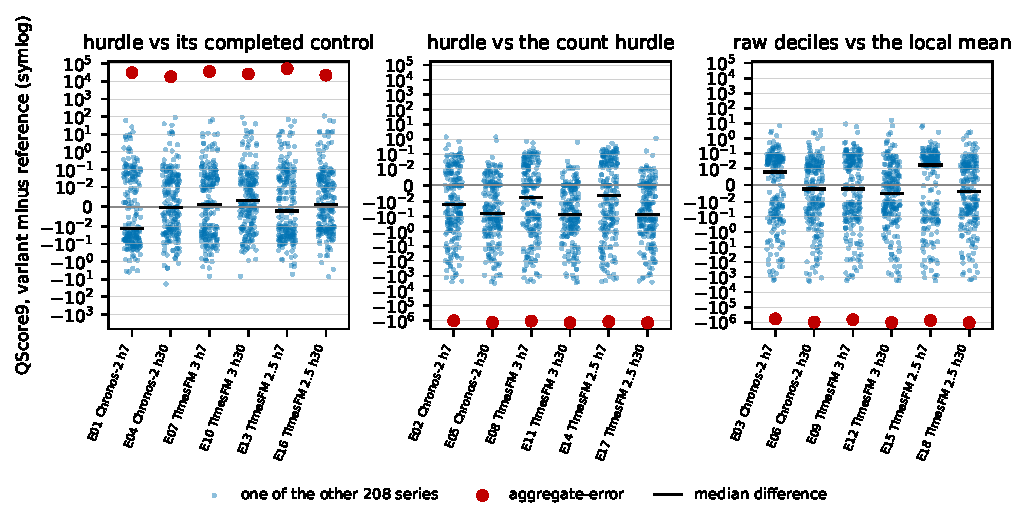
\includegraphics[width=\textwidth]{fig-s2-npm-paired-differences}
\caption{The eighteen external comparisons, series by series. Each point is one of the 209 series' paired
difference (variant minus reference \qs{}, three origins averaged) on a symmetric log scale, grouped by
contrast; the filled red marker is \texttt{aggregate-error}, and the short bar is the median. The mean of
each row, in Table~\ref{tab:s2ext}, is the red marker's value divided by 209 plus a remainder of a different
order.}
\label{fig:s2npm}
\end{figure}

\paragraph{Post-hoc: the family without the three zero days.} This paragraph is post-hoc. It was computed
on 2026-10-16 from the saved npm forecasts, after the registered scores were seen and before item 6 of the
dated addition of 2026-10-16 was written; the addition keeps the registered analysis as the default, so no
confirmatory result depends on the order. Each removed day is dropped from the one horizon-30 block that
holds it, the block is re-scored over its remaining 29 days, and the registered aggregation, test, seeded
bootstrap and one adjustment run unchanged (Appendix Table~\ref{tab:s2sens}). Without all three days, which
re-scores 10,032 forecasts, none of the eighteen conclusions changes: no row changes the side with the
larger signed-rank sum, the sign of its mean or its rejection. Without the two panel-wide days only, which
re-scores 6,688 forecasts, one conclusion changes: E06, Chronos-2's raw deciles against \lm{} at horizon 30,
no longer rejects, with adjusted $p$ 0.0599 and raw $p$ 0.0399 against 0.0119 and 0.00663 registered; it
still favors the model by rank sum, with the model lower on 110 of 209 series. Without the three days the
hurdle-against-control means at horizon 30 grow, E04 from 90.24 to 159.3, E10 from 128.5 to 201.2 and E16
from 110.3 to 183.4, and those means belong to \texttt{aggregate-error}. The mechanism answer does not
depend on the three days.

\paragraph{Post-hoc: the model's positive law with the dynamic count's occurrence.} This paragraph is
post-hoc. It was computed on 2026-10-16 from the saved forecasts of both runs, after the registered
scores were seen, with no registered status; it adds no test to E01 to E18 or S01 to S06 and replaces
nothing in them, and no model was run. The wrapper is the registered hurdle with the Jeffreys $p$
replaced by the occurrence probability of \texttt{dynamic\_count}'s saved law for the same day, the
discounted Beta-Bernoulli with discount 0.98, with $G_+$ the model's saved completed positive law exactly
as the registered hurdle uses it; it is compared with the model's completed control, its registered
hurdle, \texttt{dynamic\_count} and \hc{} in two post-hoc families, 24 tests on npm and 12 on the grid,
each with the registered settings and its own adjustment at $q = 0.05$ (Appendix
Tables~\ref{tab:s2dyn} and~\ref{tab:s2dynrest}). The dynamic occurrence shrinks the loss and removes
four of the five rejections against the substitution, and it still never beats the model's own zero mass
at $q = 0.05$: against the completed control no npm row and one grid row reject, with every mean
difference still positive; against the registered fixed-occurrence hurdle the wrapper rejects in its
favor at horizon 30 on npm and on the grid; and on the grid it has the lowest zero-day part of every
forecaster while its positive-day underprediction part stays above the completed controls' and
\texttt{dynamic\_count}'s, so with the occurrence held equal the remaining loss is the positive law
(Appendix~\ref{app:s2tables}). Study 3 carries this occurrence into a registered family
(Section~\ref{sec:s3design}).

\paragraph{Read together.} Replacing a frozen model's own zero mass with the 28-day context-only occurrence
probability, keeping the model's completed positive law, does not lower \qs{} on the pooled families, which
speak for the dense regime; by stratum the typical sparse series at horizon 7 favors the substitution, the
typical dense series favors the control, and at 30 days the strata are null. A dynamic occurrence estimate
narrows the gap and does not close it. The model's positive law beats a shifted-Poisson count hurdle in all
six npm cells and loses or is not rejected on the grid; against an empirical positive law its advantage holds
at 30 days and on dense series. The registered dynamic count beats every foundation model on the grid and
loses to them on npm. The raw deciles beat the local mean on the npm mean in every cell and on the rank test
at horizon 30 for all three models. Null, adverse, mixed and
imprecise outcomes are reported with the same care as a positive one.


\section{Discussion}
\label{sec:discussion}

\paragraph{What the two studies say together.} Study 1 found the models' mean gain against the local mean
on positive days where the local mean overpredicts, and a zero-day part against the models in every cell,
small beside the mean gain but larger than every median difference. Study 2 asked whether that zero-day loss
can be taken out by a context-only occurrence estimate while the model's size forecast is kept. It cannot be
taken out without paying more on positive days. In all nine hurdle-against-control cells of both studies the
substitution lowers the zero-day loss and the positive-day overprediction loss and raises the positive-day
underprediction loss by more than both (Table~\ref{tab:s2parts}); the net is the control's in every cell, two
of six npm tests and all three synthetic tests reject against the substitution, and no test favors it. The
occurrence Brier score, where it is lower for the hurdle (E01, E04, E13), does not carry over to the quantile
score, which couples occurrence and size: with the positive law held fixed, mass moved onto zero pulls the
lower deciles down, and on positive days those deciles underpredict. A context-only occurrence estimate does
not improve a frozen model's own completed zero mass under this score, on either the npm panel or the grid.

\paragraph{The positive law.} The second contrast isolates the model's size forecast, because both sides
share the occurrence rule and their Brier difference is exactly zero. On npm the model's completed positive
law beats the shifted Poisson fitted to the last 28 days in all six cells, on the mean, the median and the
rank test, and on the context-scaled score. On the grid it loses for two models and ties for the third
(Appendix Tables~\ref{tab:s2scores} and~\ref{tab:s2synscores} give every variant's mean score on both
panels). What
differs between the two settings is reported, not explained beyond what the accounting shows: the grid's
generator draws its positive sizes from $1 + \text{Poisson}(\mu_{+} - 1)$, the count hurdle's own family,
and the npm series do not; the npm panel spans scales from two downloads a day to millions, and the grid's
cells hold $\mu_{+}$ at 1, 5 and 25. Which of these, if any, accounts for the reversal is not something these
tests separate.

\paragraph{The raw contrast on a second domain.} On npm the raw deciles beat the local mean on the mean in
all six cells and on the rank test in four of six, with the typical series favoring the reference only at
horizon 7 for two models; in Study 1 the rank test favored the reference in all nine cells. The two panels
differ in what is counted, in scale, in sparsity (a dense stratum with few zeros against a star panel where
most days are zero for most repositories), in horizon and in calendar; the paper reports the difference and
does not attribute it. In both studies the mean is carried by few series, 88.5 to 94.3 percent of the
positive gain by five repositories in Study 1 and 0.995 to 0.998 of it by five series on npm, and in both
the mean and the typical series are shown together because they can disagree.

\paragraph{What the paper claims, and what it does not.} The literature re-check of 2026-10-12
(Section~\ref{sec:s2question}) sets the claim. The paper claims the registered combination and nothing
broader: a context-only occurrence probability substituted for the zero mass of frozen Chronos-2 and
TimesFM forecasts, their completed positive law kept, judged by a proper quantile score against a
completed-unwrapped control, matched count hurdles and a dynamic count baseline, on a probability sample of
daily attention and adoption counts, with the mean and the typical series reported side by side. It does not
claim to be the first evaluation of frozen foundation models on sparse daily counts \citep{schoess2026,
ebrahim2026}, the first hurdle applied to a frozen model's output \citep{chin2026}, or the first to show
that aggregate and per-series rankings disagree \citep{islam2026, kim2026}; a later test window on familiar
entities is not shown here to establish generalization to unseen ones \citep{moghadasi2026}, and the one
live benchmark of GitHub stargazer forecasting selects its panel by popularity where Study 1 samples a
population \citep{garza2026}. The paper does not show that the models forecast bursts, that the
substitution would fare the same on NYC 311 requests or Wikipedia pageviews, which were registered and are
not run, that any result transfers to launches or to the days after a release, or that an npm download is a
human adoption. Study 2's answer is to the registered question as registered, on the panel it achieved,
with the source's three zero days scored as served and a post-hoc sensitivity beside them.

\section{Limitations}

Study 1's limitations stand as the report gave them; Study 2 adds its own.

\begin{itemize}
\item \emph{A fetch-time survivor panel.} The 470 skips were repositories that no longer resolved publicly in
  September 2026. Equal weighting describes the panel of repositories still public with complete histories,
  not all repositories created in the window.
\item \emph{Surviving stars, not gross additions.} The endpoint reports stars that still exist at retrieval.
  In the 2024 validation the endpoint total was below the archive total for 17 of 20 repositories; for the
  15 large projects the ratio ran from 0.728 to 0.994, with 13 of 15 at least 5 percent below. The study
  target is the surviving-star history; no correction is applied, and later unstars can change the apparent
  past.
\item \emph{Los Angeles day bins.} The endpoint's day boundary was resolved to America/Los\_Angeles days by
  validation, not documented by GitHub; the validation also showed that the transition days around daylight
  saving do not uniformly favor one calendar.
\item \emph{Three windows per repository, and horizons sharing targets.} Inference is conditional on the
  fixed calendar of three cutoffs; the 7- and 30-day targets are prefixes of the 90-day targets, so the
  nine cells per reference are not independent.
\item \emph{Pointwise intervals and BH.} The bootstrap intervals are pointwise, not simultaneous, and the
  Benjamini-Hochberg adjustment carries its usual dependence assumptions.
\item \emph{The signed-rank symmetry assumption.} The Wilcoxon test's location interpretation requires
  symmetric differences, which these are not; it is reported as registered and is not a test of the mean.
\item \emph{AutoETS as a weak uncertainty reference.} Its 80 percent intervals cover about 99 percent of
  target days; a model can beat it on nearly every repository by being less wide. Read with the coverage
  results, the comparison against the local mean is the more informative of the two; that is a reading made
  after the results, and both comparisons stay reported as registered.
\item \emph{Training contamination unresolved.} No author-disclosed complete-corpus training cutoff exists
  for any of the three models; the model cards name specific sources with dates, which do not bound the
  whole corpus. What can be said is bound by availability, per model. The targets, 2025-12-05 to 2026-08-31,
  postdate the pinned TimesFM 2.5 revision, dated 2025-10-02, but are not shown to postdate the pinned
  Chronos-2 revision, dated 2026-06-05, or the pinned TimesFM 3 revision, dated 2026-09-02 with weights
  uploaded 2026-08-24; these are repository revision dates, not training cutoffs. Every repository's history
  before the cutoffs may be familiar to all three models, and a later test window on familiar entities does
  not establish generalization to unseen ones \citep{moghadasi2026}. The controls are Study 1's registered
  follow-up cohort and the lapsed October holdout; neither has run (Section~\ref{sec:notrun}).
\item \emph{The mature-phase calendar.} Every repository is forecast between nine and 41 months after
  creation. Nothing here concerns launches or the days after a release.
\item \emph{Version 1 not recomputed.} The version 1 numbers are quoted from preserved documents.

\item \emph{Three zero days in the npm targets.} The download API served 0 for all 209 series on
  2026-07-12 and 2026-08-14 and 0 for the largest series on 2026-06-25, between days of millions, and no
  context day does this. The registered completeness rule accepted them as explicit counts, the run scored
  them so, and the dated addition of 2026-10-16 keeps that analysis as the confirmatory one. These are
  properties of the source as served and of the registered rule, not of any model. The post-hoc sensitivity
  removes the days: none of the eighteen conclusions changes without all three, and one row, E06, stops
  rejecting without the two panel-wide days. Whether npm will restore the days is unknown, and nothing here
  verifies that they are gaps.
\item \emph{One series carries every npm mean.} With equal series weights on the unscaled score, as
  registered, the mean paired difference over 209 series is the difference of \texttt{aggregate-error}, at
  7.6 million downloads a day, divided by 209 plus a remainder of a different order, and the series
  bootstrap interval inherits the same dependence. Every mean in Table~\ref{tab:s2ext} is a statement about
  that series; the medians, counts, rank tests and per-stratum counts are rank-based, and the context-scaled
  score is the registered scale-free secondary. This is a property of the registered weights, stated as such.
\item \emph{The very sparse stratum holds nine series.} Only 9 of 9,998 complete candidates had zero
  downloads on at least 90 percent of the stratum window, and the registered rule forbids a larger pool, a
  transfer of slots or another filter. The family pools all 209 series as registered; every per-stratum table
  states $n = 9$, and that stratum supports no reading beyond its counts.
\item \emph{Training contamination, the npm categories.} No numerical source or entity overlap is
  established for npm by the reviewed model-card disclosures, and package-name familiarity is not evidence
  about a numerical series; training overlap remains unknown; and the target blocks of 2026-06-03 to
  2026-08-31 postdate the pinned TimesFM 2.5 revision but are not shown to postdate the pinned Chronos-2 or
  TimesFM 3 revisions, so no all-model temporal-clean claim is made. The controls that would separate
  familiarity from skill, the follow-up cohort and the holdout, have not run.
\item \emph{The synthetic grid's limits.} The generator's positive law is a shifted Poisson, the count
  hurdle's own family, so the grid is a favorable setting for the count hurdle and an unfavorable one for a
  foundation model's size forecast; its 18 cells and 30 replicates cover three zero probabilities, three
  positive means and two persistences and nothing else; its families may be familiar in kind to the models,
  which is not measurable; and no transfer to a natural domain follows from it. The oracle shows what the
  score rewards on this generator, not what any model should have done.
\item \emph{Two external domains, one horizon pair, three origins.} NYC 311 and Wikipedia are registered
  and not run, so the external result is one domain; the horizons are 7 and 30 days, the 7-day blocks are
  prefixes of the 30-day blocks, and inference is conditional on three fixed origins. The completion of a
  model's deciles into a count law is a Study 2 assumption, and the discrete CRPS is unavailable for the one
  series whose counts defeat the certified bound.
\item \emph{What a download measures.} npm counts tarball requests, including mirrors and automated
  clients; the series are a directional indicator of adoption, not a count of users, and a package that is
  rarely without a request is why the very sparse stratum is short.
\end{itemize}

\section{What is registered and not run}
\label{sec:notrun}

\paragraph{Study 1's follow-up cohort.} The protocol registers a separate follow-up on repositories created
on or after 2026-09-13, to run after this write-up with identical eligibility, strata, sample size, model
revisions, baselines, scores, regime rules and relative window calendar. It is an availability-bound
exclusion based on the already frozen checkpoints, not a claimed training cutoff; it contributes no test or
result to this report's family; and its creation-window closing date, future endpoint and frame coverage are
registered as still open, to be fixed before any follow-up collection. It has not run.


\paragraph{The October holdout.} Study 2's prospective component registered an October 2026 calendar
holdout on the frozen GitHub panel and the npm panel, with a freeze at 2026-09-28 18:00 UTC and a family of
18 tests H01 to H18. The freeze deadline passed with no freeze plan prepared, no forecast generated and no
prediction committed; under the registered rule a late commit fails the prospective gate and no backdating
is allowed. The dated addition of 2026-10-12, item 1, records the holdout as registered and not run, with no
result and no settlement retrieval. A holdout on possibly familiar entities would in any case not replace
Study 1's follow-up cohort or show generalization to unseen ones \citep{moghadasi2026}.

\paragraph{NYC 311 and Wikipedia.} The registered external component had three domains. The dated addition
of 2026-10-12, item 3, decided before any Study 2 target value was accessed, fixes this paper's external
family as the eighteen packages-domain tests E01 to E18 and defers NYC 311 requests and English Wikipedia
pageviews to a later run, where tests E19 to E54 keep their registered definitions and form one family of 36
with its own single adjustment; they are not merged back into a 54-test correction after the eighteen have
been seen. Nothing is claimed about either domain.

\paragraph{The November prospective round.} A November 2026 prospective round was considered and not
registered; it would need its own dated addition before its freeze. Nothing is claimed about it.

\section{Reproducibility}

The repository \url{https://github.com/vprchlik/PulseGraph} contains the study code, the offline tests, the
protocol with its dated additions, the declarations under \texttt{study/} and the evidence package under
\texttt{reports/registered-2026-09-13/}, from the frozen manifest and daily signals to the confirmatory
inference tables and the post-hoc accounting; Appendix~\ref{app:repro} lists what it holds and does not hold,
the commands that regenerate every table, the hardware and package versions of the run, and the licences.
The complete results file \texttt{results.parquet} (433,172,286 bytes, SHA-256
\texttt{53ff5a5316fd43dd898866c4fc54edf913b080a32cbd696d7e3b3fc528f62df6}) holds every forecast, quantile
grid, context, target and seed. It is to be published as a GitHub release asset; the URL is to be filled by
the author at posting and is marked in the repository's README.


Study 2's two runs are under \texttt{reports/study2-synthetic-2026-10-15/} and
\texttt{reports/study2-npm/run-2026-10-15/}: each holds the run's state with the SHA-256 of every
checkpoint, the readiness, the implementation commit and source hashes, the package versions and the
hardware; the inference directory with the family table, the per-entity paired differences, the secondary
tables, the PIT histograms and a provenance file; the results document and the script that prints its tables
from the inference files; and a provenance file with the SHA-256 of every file in the directory and of the
inputs. The synthetic directory adds the per-row score recomputation and its output; the npm directory adds
the integrity check's outputs, the target pull's ledger and completeness document, the per-day summary of the
targets with the script that writes it, the script that reproduces each test's direction and raw $p$ from
the paired differences, and the post-hoc directory with the sensitivity command, its outputs and its
provenance. The 540 synthetic checkpoints (about 0.9 GB) and the 209 npm checkpoints (338 MB), one JSON
file per series with every forecast, are not in the tree; their SHA-256 values are in each run's state file,
and they are to be published as release assets beside \texttt{results.parquet}, so that a fresh clone can
rerun the inference, the integrity recomputation and the sensitivity. The npm context and target captures
stay in the ignored raw directory with their hashes in the completeness document; the panel's manifest and
selection files are in the tree, and the aggregated daily counts of the 209 series are published with the
paper under the data statement of Appendix~\ref{app:s2panel}. Appendix~\ref{app:s2repro} lists the
commands.

\section{How this work was made}

The following is the author's own statement, as it stands in the repository's README.

\begin{quote}
This study exists for three reasons: the question, whether zero-shot time-series foundation models improve
probabilistic forecasts of sparse daily counts; the audit of its first version, which found no invalidating
code defect but two design flaws; and the registered redesign that answers the question without them. The
code in this repository was written with AI coding agents under my direction. I set the question, registered
the protocol before any target data was fetched, ran the studies on my own machine, and made the decisions
that the protocol and the evidence package record as the author's. Every number in \texttt{RESULTS.md} traces
to a saved file under \texttt{reports/} and to the command that regenerates it, named in this README and in
\texttt{RESULTS.md}.
\end{quote}


\bibliographystyle{plainnat}
\bibliography{references}

\appendix

\section{The registered design, the remaining detail}
\label{app:design}

\paragraph{Count source and validation.} Daily counts come from GitHub's star-history endpoint
\citep{github-star-history-2026, github-api-star-history}, released 2026-09-04, from creation through the
common endpoint 2026-08-31. GH Archive supplies the frame, not the counts, because its WatchEvent capture
degraded from mid-2025 \citep{gharchive-issue-320}. Before the freeze, 20 validation repositories created
before 2023 (and so outside the study frame) were fetched and compared hourly with deduplicated GH Archive
WatchEvents over 2024. Over the 365 matched days, America/Los\_Angeles calendar days with daylight saving gave
the lowest mean absolute daily difference for 20 of 20 repositories against UTC and 18 of 20 against fixed
UTC$-$8, with two repositories tied between the Los Angeles and fixed-offset calendars (pooled mean absolute
difference 1.975 against 2.065 and 2.713); the author accepted Los Angeles days as the calendar. The endpoint
reports stars that still exist at retrieval, dated by when they were given: the 2024 endpoint total is below
the archive total for 17 of 20 repositories. The target is therefore the surviving-star daily history as
retrieved in September 2026, not gross additions.

\paragraph{Calendar.} The common endpoint $E$ is 2026-08-31. Cutoffs are $c_j = E - (j \times 90 - 1)$
days for $j = 3, 2, 1$: 2025-12-05, 2026-03-05 and 2026-06-03. Context ends the day before the cutoff;
targets run from the cutoff for 7, 30 or 90 days. The three 90-day windows partition the trailing 270 days
and do not overlap; shorter horizons use the same cutoffs, so horizons share targets and are not independent.
Every model has at least 90 context days, uses only the repository's own history, and refits (for the
baselines) on context only.

\paragraph{Regimes.} Three context-only labels, descriptive and pooled for inference: ``inactive recently''
when the 28 days before the cutoff sum to zero; ``recent surge'' when the last seven days hold at least seven
stars and their daily rate is at least three times the larger of the preceding four weeks' daily rate and one;
``other active'' otherwise. Tests perturb, permute and extend data on and after each cutoff and assert
unchanged labels and strata.

\paragraph{Models.} Three frozen foundation models with exact repository revisions:
\texttt{amazon/chronos-2} at \texttt{29ec3766d36d6f73f0696f85560a422f50e8498c} (weights and package
Apache-2.0) \citep{chronos2-weights, chronos2-2025};
\texttt{google/timesfm-3.0-pytorch} at \texttt{43046b85ec22d584a13f8098c2ed39c889e129c2} (weights under the
TimesFM Non-Commercial License v1.0, package Apache-2.0) \citep{timesfm3-card, timesfm-license};
\texttt{google/timesfm-2.5-200m-pytorch} at \texttt{1d952420fba87f3c6dee4f240de0f1a0fbc790e3} (Apache-2.0)
\citep{timesfm25-card}. All run univariate, batch size one, a 2,048-day maximum context, on one GPU. Two
primary references: \lm{}, the mean of the last 28 context days with 200 empirical context-level draws, and
\aets{}, StatsForecast AutoETS with season length 7 and native intervals \citep{statsforecast-2.1.1}. Thirteen
secondary baselines: AutoARIMA and AutoTheta with weekly season, a negative-binomial local level with a 28-day
mean and context-moment dispersion, local means with lookbacks 7, 14, 56 and 90, and the version 1 families
(last value, weekly naive, horizon-dependent seasonal naive, 30-day linear trend, nonseasonal Holt, LightGBM).

\paragraph{Score.} The primary score is \qs{}, twice the mean pinball loss over the nine deciles
$\tau \in \{0.1, \dots, 0.9\}$ and the $h$ target days,
\[
\qs{} = \frac{2}{9h} \sum_{t=1}^{h} \sum_{\tau} \max\{\tau (y_t - q_{t,\tau}),\, (\tau - 1)(y_t - q_{t,\tau})\},
\]
defined for all-zero targets and equal to the weighted interval score at the matching levels
\citep{bracher2021}; it is a proper score for the nine quantiles \citep{gneiting2007}. Deciles are native or
analytic where a model supplies them and linear empirical quantiles of 200 draws otherwise; negative
forecasts are clipped to zero and crossings repaired by cumulative maxima, with both repairs recorded. No
tails beyond the supported deciles are invented for either TimesFM.

\paragraph{Inference.} Window scores are averaged within repository and horizon, then repositories are
weighted equally. For each of the 18 declared comparisons (three models, two references, three horizons)
the paired difference $d$ is model minus reference, so negative favors the model. The mean of $d$ carries a
pointwise 95 percent percentile interval from 20,000 bootstrap replicates of whole repositories (seed
20260914). A two-sided approximate Wilcoxon signed-rank test across repository averages, omitting zero
differences, tests a zero-centered symmetric null; its location interpretation requires symmetry and it is
not a test of the mean. Benjamini-Hochberg adjustment is applied once at $q = 0.05$ over the 18 tests, with
its usual dependence assumptions. Strata, regimes, other lookbacks, calibration and the scale review are
declared secondary and add no test. Seeds: selection 20260913, forecast 20260912, bootstrap 20260914.


\section{Version 1: the disclosure list and the local-mean table}
\label{app:v1}

The audit listed what version 1 had to disclose: a weak original baseline set; Wilcoxon tests on overlapping
windows treated as independent; untested scale domination; a mislabeled 95 percent interval for TimesFM,
whose API exposes only the 0.1 to 0.9 quantiles; ordinary PIT on discrete counts; unseeded baseline sampling;
LightGBM's uncertainty from in-sample residuals; MAPE as a headline metric on zero-inflated series; implicit
observation endpoints that censored trailing zeros and omitted later-removed stars; and unresolved
pretraining contamination with no clean post-release holdout. Every version 1 number in this report is
quoted from the preserved version 1 documents (its results document, its audit and its write-up, with four
figures), not recomputed. The version 1 result artifacts (the results parquet, the summary CSV, the review
outputs and the raw stargazer data) were excluded from that repository by its ignore rules and exist only on
a computer the author no longer uses; their recovery is deferred.

\begin{table}[h]
\centering\small
\caption{Version 1, quoted from the preserved documents: mean CRPS of the 28-day local mean added by the
audit and of the two foundation models, by discovery cohort and horizon. These numbers were not recomputed;
the version 1 artifacts are on a computer the author no longer uses.}
\label{tab:v1}
\begin{tabular}{llrrr}
\toprule
Cohort & Horizon (days) & Local mean & Chronos-2 & TimesFM-2.5 \\
\midrule
breakout-selected & 7 & 7.77 & 6.43 & 6.23 \\
breakout-selected & 30 & 8.77 & 7.90 & 7.68 \\
breakout-selected & 90 & 9.41 & 8.52 & 8.20 \\
steady-selected & 7 & 1.66 & 1.46 & 1.44 \\
steady-selected & 30 & 2.26 & 2.04 & 2.02 \\
steady-selected & 90 & 2.42 & 2.21 & 2.22 \\
dead-selected & 7 & 2.75 & 2.43 & 2.35 \\
dead-selected & 30 & 2.64 & 2.47 & 2.39 \\
dead-selected & 90 & 2.85 & 2.73 & 2.67 \\
\bottomrule
\end{tabular}
\end{table}


\section{Reproducibility, the detail}
\label{app:repro}

\paragraph{What a fresh clone holds.} The repository contains the study code, the offline tests, the
protocol with its dated additions, the declarations under \texttt{study/} (the 18 comparisons, the run
specification with model revisions, the 20 validation repositories, both SQL queries), and the evidence
package under \texttt{reports/registered-2026-09-13/}: the frozen manifest and aggregate daily signals, the
full eligible frame and its frozen order, the skip log, the query exports and provenance, the hourly
validation comparison and figures, the signed readiness review, the run metadata with package versions and
hardware, the integrity log, the confirmatory inference tables, the declared descriptive tables and the
post-hoc accounting. It does not contain raw endpoint responses, model weights, the version 1 reference copy,
or the private research notes. The BigQuery frame and validation queries billed 12,510,623,170,560 bytes
(about \$71.11 at the list price before credits), approved in writing before they ran.

\paragraph{Commands.} Place the release asset at
\texttt{reports/registered-2026-09-13/run/results.parquet}, then from the repository root, with the
project's Python environment:
{\footnotesize
\begin{verbatim}
.\.venv\Scripts\python.exe -m scripts.review_integrity --run reports/registered-2026-09-13/run
.\.venv\Scripts\python.exe -m scripts.registered_inference --run reports/registered-2026-09-13/run `
    --out data/cache/inference-reproduction
.\.venv\Scripts\python.exe reports/registered-2026-09-13/summarize_descriptives.py
\end{verbatim}}
The first verifies hashes, the grid, contexts, targets, labels, seeds and recomputes every score; the second
regenerates the 18-row inference table from the saved forecasts without refitting; the third regenerates the
descriptive CSVs behind the tables of Appendix~\ref{app:tables}. The post-hoc accounting is regenerated by
\texttt{reports/registered-2026-09-13/posthoc/accounting.py}, and the figures of this report by
\texttt{paper/figures/make\_figures.py}, which reads only the saved CSVs. The run itself used an NVIDIA
GeForce RTX 4070 SUPER (driver 610.47, CUDA 12.8, PyTorch 2.11.0), \texttt{chronos-forecasting} 2.3.2,
\texttt{timesfm} 3.0.2 and \texttt{statsforecast} 2.1.1 \citep{timesfm-pypi, statsforecast-2.1.1}.

\paragraph{Licences.} The code is MIT. The aggregate dataset and this write-up are CC BY 4.0. Chronos-2 and
TimesFM 2.5 weights are Apache-2.0; TimesFM 3 weights carry the TimesFM Non-Commercial License v1.0; the
Chronos and TimesFM packages are Apache-2.0.


\section{Additional tables and figure}
\label{app:tables}

\begin{table}[h]
\centering\small
\caption{AutoETS interval coverage and 90-day widths by stratum. Coverage is a declared secondary summary:
inclusive coverage of the repaired 0.1 to 0.9 quantiles at each horizon. The widths and the specification
counts were requested after the run, within the declared secondary calibration analysis. Widths are the
median over fits of the 90-day daily width and the median of the fit-mean width, both after clipping and
crossing repair. The last column counts fits that selected multiplicative seasonality, at each horizon.}
\label{tab:autoets}
\begin{tabular}{lrrrrrr}
\toprule
Stratum & Cov.\ $h=7$ & $h=30$ & $h=90$ & Daily width & Fit-mean width & Mult.\ fits \\
\midrule
20--99 & 0.979 & 0.978 & 0.980 & 0.79 & 0.80 & 0 \\
100--999 & 0.991 & 0.988 & 0.989 & 3.60 & 3.71 & 0 \\
1000+ & 0.991 & 0.994 & 0.995 & 49.69 & 55.99 & 6 \\
\bottomrule
\end{tabular}
\end{table}

\begin{table}[h]
\centering\small
\caption{Pooled \qs{} by day-90 stratum and horizon, declared secondary: three windows averaged within
repository, then 100 repositories per stratum weighted equally. These are stratum means; the typical
repository by stratum is given, labeled post-hoc, in Section~\ref{sec:results}.}
\label{tab:stratum}
\begin{tabular}{llrrrrr}
\toprule
Stratum & $h$ & Chronos-2 & TimesFM 3 & TimesFM 2.5 & \lm{} & \aets{} \\
\midrule
20-99 & 7 & 0.077 & 0.077 & 0.079 & 0.075 & 0.148 \\
20-99 & 30 & 0.084 & 0.084 & 0.085 & 0.082 & 0.162 \\
20-99 & 90 & 0.086 & 0.101 & 0.088 & 0.083 & 0.189 \\
100-999 & 7 & 0.217 & 0.219 & 0.226 & 0.228 & 0.542 \\
100-999 & 30 & 0.217 & 0.215 & 0.221 & 0.217 & 0.703 \\
100-999 & 90 & 0.233 & 0.231 & 0.235 & 0.236 & 0.967 \\
1000+ & 7 & 2.798 & 2.432 & 2.470 & 3.200 & 5.609 \\
1000+ & 30 & 3.134 & 2.929 & 2.923 & 3.531 & 8.950 \\
1000+ & 90 & 3.966 & 3.874 & 3.930 & 4.270 & 23.301 \\
\bottomrule
\end{tabular}
\end{table}

\begin{table}[h]
\centering\small
\caption{Inclusive 80 percent coverage of the repaired 0.1 to 0.9 quantiles, averaged within repository and
then over 300 repositories, declared secondary.}
\label{tab:calibration}
\begin{tabular}{lrrr}
\toprule
Model & $h=7$ & $h=30$ & $h=90$ \\
\midrule
chronos2 & 0.832 & 0.824 & 0.837 \\
timesfm3 & 0.880 & 0.910 & 0.889 \\
timesfm2p5 & 0.924 & 0.906 & 0.918 \\
local\_mean\_28 & 0.955 & 0.945 & 0.941 \\
autoets\_weekly & 0.987 & 0.986 & 0.988 \\
\bottomrule
\end{tabular}
\end{table}

\begin{table}[h]
\centering\small
\caption{The declared scale review against \lm{}. The top-five share divides the five largest positive
repository gains (reference minus model) by all positive gains. Skill, $1 - \text{model}/\text{reference}$,
is undefined where the reference's loss is zero. The leave-one-out range is the mean gain with each
repository removed in turn.}
\label{tab:scale}
\begin{tabular}{llrrc}
\toprule
Model & $h$ & Top-five share of positive gain & Skill defined (of 300) & Leave-one-out mean gain \\
\midrule
Chronos-2 & 7 & 0.902 & 209 & [0.060, 0.152] \\
Chronos-2 & 30 & 0.910 & 239 & [0.074, 0.134] \\
Chronos-2 & 90 & 0.892 & 259 & [0.068, 0.105] \\
TimesFM 3 & 7 & 0.932 & 209 & [0.066, 0.280] \\
TimesFM 3 & 30 & 0.929 & 239 & [0.083, 0.203] \\
TimesFM 3 & 90 & 0.895 & 259 & [0.064, 0.133] \\
TimesFM 2.5 & 7 & 0.943 & 209 & [0.049, 0.265] \\
TimesFM 2.5 & 30 & 0.943 & 239 & [0.073, 0.203] \\
TimesFM 2.5 & 90 & 0.885 & 259 & [0.046, 0.120] \\
\bottomrule
\end{tabular}
\end{table}

\begin{figure}[h]
\centering
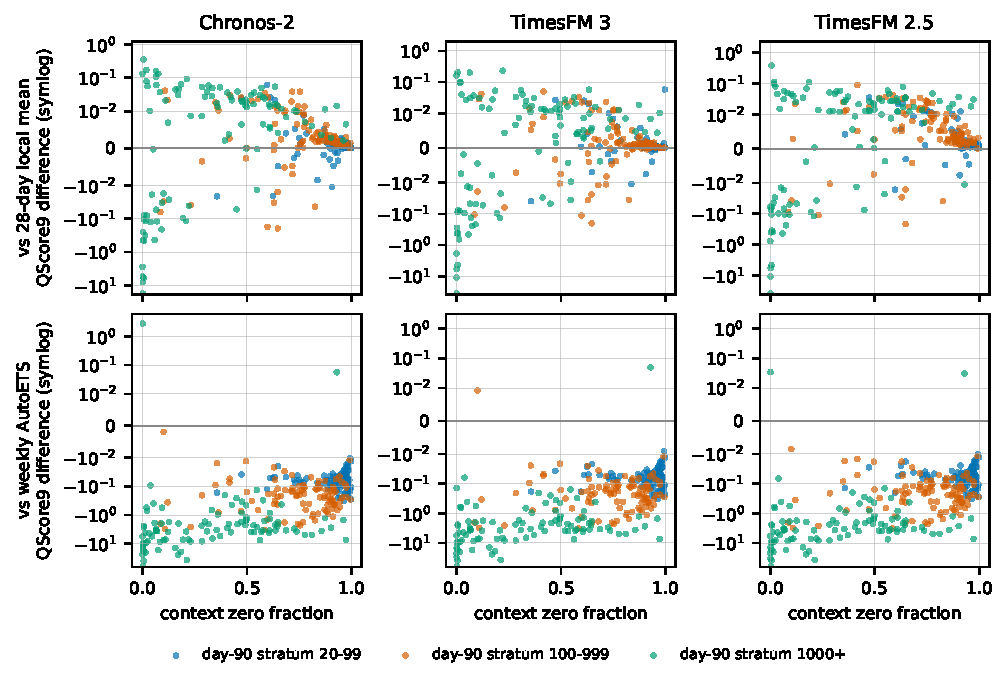
\includegraphics[width=\textwidth]{fig-posthoc-zero-fraction-h30}
\caption{Post-hoc. Each repository's paired difference at horizon 30 against the fraction of zero days in
its context (three windows averaged), colored by day-90 stratum, on a symmetric log scale. Top row: against
\lm{}; bottom row: against \aets{}. Against the local mean the large model gains are at low zero fractions
and the small model losses cluster at high ones; against AutoETS nearly every repository at every zero
fraction favors the model.}
\label{fig:zerofraction}
\end{figure}


% Study 2, the registered design, the remaining detail: the paragraphs moved from study2-design.tex so
% that the body stays at the report's length. Input from paper.tex in the appendix; every number traces to
% sources.md and is asserted by check_numbers.py.
\providecommand{\lm}{\texttt{local\_mean\_28}}
\providecommand{\aets}{\texttt{autoets\_weekly}}
\providecommand{\qs}{QScore9}
\providecommand{\hc}{\texttt{hurdle\_count\_28}}

\section{Study 2: the registered design, the remaining detail}
\label{app:s2design}

\paragraph{Scores.} \qs{} is primary, as in Study 1: twice the mean pinball loss over the nine deciles and
all target days, averaged over origins within series and horizon, with every series then weighted equally
within its domain; domains are never pooled. Four secondary scores are declared. The scaled score divides
each window's \qs{} by $\max(1, \bar{y}_{\text{context}})$, the mean of the full allowed context, before the
same averaging. The occurrence Brier score is $(p - \mathbf{1}[y > 0])^2$. The discrete CRPS is
$\sum_{k \ge 0} (F(k) - \mathbf{1}[y \le k])^2$ for a forecast with an integer-supported distribution of
finite first moment; the registered numerical rule requires a certified residual bound below $10^{-8}$ by
$k = 1{,}000{,}000$ and forbids truncation or a sampled substitute. The addition of 2026-10-15 fixes what
happens when that bound is not attained: the forecast's CRPS is recorded as unavailable with that reason and
counted in the valid denominators the protocol already requires, and the run continues; the limit, the
tolerance and the certification are unchanged. The case that prompted it is one npm series whose context
runs into the millions a day (Section~\ref{sec:s2panel}), identified from the frozen context alone before
any target was opened. The randomized PIT draws one recorded uniform within each CDF jump and gives
calibration histograms with no significance claim. Raw native deciles have no identified occurrence
probability and no full CDF, so their Brier, CRPS and PIT fields are unavailable by construction; AutoETS's
continuous intervals are not forced through the integer sum. Every secondary score reports its availability
and its denominator. The three exact accounting parts of Study 1's post-hoc accounting (Table~\ref{tab:posthoc}) are
reported for every comparison with the full horizon denominator.

\paragraph{Seeds, provenance and the gate.} Six root seeds are registered: selection 20260914, forecasts
20260915, PIT 20260916, bootstrap 20260917, synthetic 20260918 and prospective 20260919; every stream is
derived from its root through SHA-256 of canonical identifiers, never from a process-randomized hash, and
each derived stream is recorded. Before a component runs, its gate requires the Study 2 registration commit
and the full protocol hash at that commit, the unchanged Study 1 bytes, the exact implementation commit and
source hashes, package versions and model revisions, the complete ordered manifest, the seeds, the calendar
and source semantics, the approved extraction budget and runtime, and a GPU smoke of the current
implementation; it validates the comparison lists as declared and refuses an unresolved family, a missing
seed, an unpinned model or a missing registration. For this paper's external component the gate, changed in
a commit that cites the addition of 2026-10-12, requires one npm panel bound by hash to the frozen panel
files and no holdout freeze; the registered 54-test component and its three-panel requirement are unchanged.
Leakage tests perturb, permute and extend every series on and after each cutoff and assert, with an
observed-date spy, unchanged selection, strata, scales and forecasts. Models stay resident per invocation,
whole series are checkpointed, a failed window stops the run, and a resume re-attempts the failure rather
than skipping it, under Study 1's batch-one, under-8-GB discipline on the same GPU.

\paragraph{The holdout, registered and not run.} The prospective component froze nothing. It registered an
October 2026 calendar holdout on the unchanged Study 1 GitHub panel and the accepted npm panel: a freeze at
2026-09-28 18:00 UTC of weights, transformations, baselines, manifests and forecast arrays with committed
hashes before the first target day, target blocks of October 1 to 7 and October 1 to 30, settlement
retrievals from 2026-10-15 and 2026-11-07, and a family of 18 tests H01 to H18 at horizon 30 with one
correction. The freeze deadline passed with no freeze plan, no approval, no forecast and no committed
prediction; under the registered rule a late commit fails the prospective gate and no backdating or
reconstruction is allowed, so the addition of 2026-10-12 records the holdout as registered and not run, with
no result and no settlement retrieval. The same addition resets the npm readiness clock once, to 2026-10-20
23:59 UTC, because inactivity is not the source failure the PyPI rule names; the clock was met
(Section~\ref{sec:s2panel}).

\paragraph{Contamination.} The protocol keeps three categories for every domain and component: known
source or entity overlap, unknown overlap, and whether the targets fall after the frozen checkpoints were
available. For npm, no numerical source or entity overlap is established by the reviewed model-card
disclosures, and package-name familiarity is not evidence about a numerical series; training overlap
remains unknown; and the retrospective target blocks of 2026-06-03 to 2026-08-31 are mixed by model
availability, since they postdate the pinned TimesFM 2.5 revision but are not shown to postdate the pinned
Chronos-2 or TimesFM 3 revisions, so no all-model temporal-clean claim is made. For the synthetic component,
the generator families may be familiar in kind and that familiarity is not measurable; the realizations are
new, seeded and generated after the weights were frozen, and no transfer claim to a natural domain follows
from them. No author-disclosed complete-corpus training cutoff exists for any of the three models.


% Study 2, the npm panel, the remaining detail: the paragraphs moved from study2-panel.tex so that the
% body stays at the report's length. Input from paper.tex in the appendix; every number traces to
% sources.md and is asserted by check_numbers.py.
\providecommand{\qs}{QScore9}

\section{The npm panel: the pull's budget and the data statement}
\label{app:s2panel}

\paragraph{The pull's budget and the API's limits.} The approval was 36,000 requests and 13 hours,
cumulative over the inventory, the walk and the context pull. The pull used 30,198 HTTP attempts: 12,943 to
the registry host, 12,762 to the download-counts host and 4,493 to the replication host, over 52
invocations totalling 45,508 seconds (12 hours and 38 minutes), from 2026-10-14 00:23 UTC to 2026-10-15 01:57
UTC. Attempts were spaced at least one second apart, and at least three seconds from 2026-10-14 22:51 UTC,
when the download API was answering about 20 requests a minute. The download API returned 429 to 2,708
attempts; three in a row for one key stopped the invocation, which resumed later from the saved captures.
From 2026-10-14 08:44 UTC the download API timed out or answered 504 until at least 10:25 UTC and answered
again at 21:37 UTC; each such stop wrote nothing and excluded no candidate. No documented request quota for
the download-counts API was found in the governing documents, and 30,198 attempts in about 26 hours is far
below the one stated line, five million requests a month; the redistribution review records the 429 answers
as the pull repeatedly reaching npm's throttle and honouring it.

\paragraph{Data statement.} The daily counts of the 209 series were obtained from the npm download-counts
API, \url{https://api.npmjs.org/downloads/range}, between 2026-10-14 and 2026-10-15 UTC, for 2025-09-01 to
2026-06-02; the targets for 2026-06-03 to 2026-08-31 were obtained from the same API on 2026-10-15 under a separate
target-access approval (Section~\ref{sec:s2results}). Package names and creation timestamps come from the npm public registry,
\url{https://registry.npmjs.org}, and from its replication feed, \url{https://replicate.npmjs.com}. A
download is a tarball request as npm counts it, including mirrors, build servers and automated clients, and
is a directional indicator rather than a count of users. npm, Inc.\ states no licence for the download
counts, and its Open-Source Terms of 2022-03-10, read as governing the public registry and its public APIs,
contain no restriction on their redistribution; replication of registry data through the public
APIs is expressly allowed. Names are as the registry served them at acquisition and may since have been
removed. The pull reached npm's rate limit 2,708 times and honoured it. The project's compilation of the
selection, the derived fields and the documentation is released under CC BY 4.0; no licence is asserted over
the counts as such. Maintainer names, e-mail addresses, descriptions and raw registry documents are not
published. The manifest and selection files are in the repository; the aggregated daily counts are
published with the paper. npm is a registered trademark of npm, Inc.; no npm logo is used.


\section{Study 2 reproducibility, the detail}
\label{app:s2repro}

\paragraph{What was run, and when.} The synthetic gate passed at 2026-10-15 20:16 UTC against the signed
readiness, the GPU smoke at the implementation commit and the committed grid manifest, whose generated copy
equals it; the run and its inference followed, the inference at a HEAD that differs from the implementation
commit only under the documentation directory, with no uncommitted change under the scripts or the package.
The npm gate passed twice, at 23:14 UTC before any target request and at 23:26 UTC with the pulled signals
and their completeness document; the run, the inference and the integrity check followed with HEAD at the
implementation commit and no uncommitted change. The zero-day sensitivity ran on 2026-10-16 at HEAD
\texttt{e41fdf2} with no uncommitted change under the inference script or the package. NumPy 2.5.3, SciPy
1.18.1 and pandas 2.3.3 were used throughout; each provenance file records this.

\paragraph{Commands.} Place the release assets, the checkpoints, in the two run directories, then from the
repository root with the project's Python environment (PowerShell; a completed run directory is immutable,
so the inference, integrity and sensitivity commands write to a new directory):
{\footnotesize
\begin{verbatim}
.\.venv\Scripts\python.exe scripts\study2_inference.py synthetic `
    --run reports\study2-synthetic-2026-10-15 --out <new directory>
.\.venv\Scripts\python.exe reports\study2-synthetic-2026-10-15\recompute_scores.py `
    reports\study2-synthetic-2026-10-15 --out <new file>
.\.venv\Scripts\python.exe reports\study2-synthetic-2026-10-15\make_tables.py `
    reports\study2-synthetic-2026-10-15\inference
.\.venv\Scripts\python.exe scripts\study2_inference.py external_packages `
    --run reports\study2-npm\run-2026-10-15 --out <new directory>
.\.venv\Scripts\python.exe scripts\study2_integrity.py external_packages `
    --run reports\study2-npm\run-2026-10-15 --out <new directory>
.\.venv\Scripts\python.exe reports\study2-npm\run-2026-10-15\make_tables.py `
    reports\study2-npm\run-2026-10-15\inference
.\.venv\Scripts\python.exe reports\study2-npm\run-2026-10-15\check_directions.py `
    reports\study2-npm\run-2026-10-15\inference
.\.venv\Scripts\python.exe reports\study2-npm\run-2026-10-15\posthoc\sensitivity_zero_days.py `
    reports\study2-npm\run-2026-10-15 --out <new directory>
.\.venv\Scripts\python.exe paper\figures\make_figures.py
.\.venv\Scripts\python.exe paper\check_numbers.py
\end{verbatim}}
The first regenerates the synthetic family and its secondary tables from the saved forecasts without
refitting; the second recomputes every saved synthetic score; the third prints the synthetic results
document's tables; the fourth to seventh do the same for the npm run, the integrity check recomputing every
score and verifying every checkpoint hash; the eighth re-scores the saved npm forecasts without the three
zero days; the ninth draws the five figures of this paper from the saved CSVs; the tenth asserts every
number in this paper against the files that \texttt{paper/sources.md} names. The runs themselves, the gate,
the target pull and the panel pull are not to be repeated: the gate and the pull pass only at the
implementation commit with the readiness files in place, the pull refuses to write a second snapshot, and a
new target request needs its own approval. A reader who recomputes a test from the CSVs should parse the
floats exactly (pandas \texttt{float\_precision="round\_trip"}); the default parser can move a last digit
and change a rank tie.

% Study 2, the secondary tables of the appendix, from the inference and post-hoc files of the two runs and
% the post-hoc dynamic-occurrence directory. Input from paper.tex; every number traces to sources.md and is
% asserted by check_numbers.py.
\providecommand{\lm}{\texttt{local\_mean\_28}}
\providecommand{\aets}{\texttt{autoets\_weekly}}
\providecommand{\qs}{QScore9}
\providecommand{\hc}{\texttt{hurdle\_count\_28}}

\section{Study 2: the two families, the secondary tables and the post-hoc readings}
\label{app:s2tables}

Tables~\ref{tab:s2ext} and~\ref{tab:s2syn} give the two registered families of Study 2 with every column,
the eighteen external comparisons on the npm panel and the six synthetic comparisons at horizon 30;
Figure~\ref{fig:s2npm} shows the 209 paired differences behind each external row, and
Table~\ref{tab:s2parts} splits each hurdle-minus-control difference into the three exact accounting parts.
Twelve of the eighteen external tests and five of the six synthetic tests reject at $q = 0.05$ after one
adjustment per family; of the twelve, ten reject for the model variant and two against it, and all five
synthetic rejections are against the hurdle variant. None of the other tables in this appendix carries a
multiplicity adjustment except the two post-hoc dynamic-occurrence families, which carry their own, and
none replaces the two families. Differences are model variant minus reference, so negative favors the
variant. A median of order $10^{-9}$ is a near-zero score difference repeated across series, not a tie; under
the declared rule only an exact zero is a tie.

\begin{table}[htbp]
\centering\footnotesize\setlength{\tabcolsep}{3pt}
\caption{The eighteen declared external comparisons on the npm panel. Differences are model variant minus
reference \qs{}, averaged over three origins within series and then over 209 series; negative favors the
variant. The contrast names the pair: the model's hurdle against its completed control, the hurdle against
\hc{}, or the raw deciles against \lm{} (the full tuples are in Appendix Table~\ref{tab:s2family}). The
interval is the pointwise 95 percent percentile interval from 20,000 series-cluster bootstrap replicates.
``Lower / tied / higher'' counts the series (of 209) where the variant's score is below, equal to or above
the reference's. $p$ is the Benjamini-Hochberg adjusted two-sided Wilcoxon signed-rank $p$-value over the
18 tests. Every mean in this table is carried by the series \texttt{aggregate-error}
(Appendix~\ref{app:s2panel}); the medians, counts and tests are rank-based and describe the typical series.}
\label{tab:s2ext}
\begin{tabular}{lllrrcrcl}
\toprule
ID & Model & Contrast & $h$ & Mean & 95\% interval & Median & Lower / tied / higher & Adjusted $p$ \\
\midrule
E01 & Chronos-2 & hurdle vs completed & 7 & 152 & [0.1846, 455.2] & -0.01376 & 121 / 2 / 86 & 0.203 \\
E02 & Chronos-2 & hurdle vs count hurdle & 7 & -5,090 & [-15,175, -31.08] & -0.01587 & 129 / 12 / 68 & $3.72 \times 10^{-11}$ \\
E03 & Chronos-2 & raw vs local mean & 7 & -2,884 & [-8,601, -17.33] & 0.007856 & 92 / 0 / 117 & 0.596 \\
E04 & Chronos-2 & hurdle vs completed & 30 & 90.24 & [0.2273, 269.7] & -0.0002469 & 105 / 2 / 102 & 0.449 \\
E05 & Chronos-2 & hurdle vs count hurdle & 30 & -6,563 & [-19,596, -30.03] & -0.06173 & 150 / 9 / 50 & $7.06 \times 10^{-21}$ \\
E06 & Chronos-2 & raw vs local mean & 30 & -4,734 & [-14,149, -15.84] & -0.002372 & 112 / 0 / 97 & 0.0119 \\
E07 & TimesFM 3 & hurdle vs completed & 7 & 176.9 & [0.2669, 529.4] & 0.001058 & 94 / 8 / 107 & 0.236 \\
E08 & TimesFM 3 & hurdle vs count hurdle & 7 & -5,416 & [-16,153, -31.67] & -0.007407 & 116 / 18 / 75 & $3.61 \times 10^{-8}$ \\
E09 & TimesFM 3 & raw vs local mean & 7 & -3,235 & [-9,650, -18.24] & -0.002297 & 112 / 1 / 96 & 0.0438 \\
E10 & TimesFM 3 & hurdle vs completed & 30 & 128.5 & [0.5058, 383.8] & 0.00321 & 81 / 8 / 120 & 0.00215 \\
E11 & TimesFM 3 & hurdle vs count hurdle & 30 & -6,792 & [-20,280, -31.3] & -0.0716 & 161 / 17 / 31 & $3.19 \times 10^{-25}$ \\
E12 & TimesFM 3 & raw vs local mean & 30 & -5,001 & [-14,947, -16.86] & -0.005016 & 125 / 1 / 83 & $3.82 \times 10^{-5}$ \\
E13 & TimesFM 2.5 & hurdle vs completed & 7 & 253.9 & [0.5046, 759.9] & -0.002116 & 109 / 3 / 97 & 0.628 \\
E14 & TimesFM 2.5 & hurdle vs count hurdle & 7 & -5,847 & [-17,446, -30.83] & -0.006349 & 115 / 7 / 87 & $2.66 \times 10^{-5}$ \\
E15 & TimesFM 2.5 & raw vs local mean & 7 & -3,743 & [-11,179, -17.41] & 0.01696 & 84 / 1 / 124 & 0.746 \\
E16 & TimesFM 2.5 & hurdle vs completed & 30 & 110.3 & [0.6883, 328.7] & 0.0009877 & 101 / 1 / 107 & 0.0276 \\
E17 & TimesFM 2.5 & hurdle vs count hurdle & 30 & -6,918 & [-20,665, -29.9] & -0.06938 & 160 / 9 / 40 & $1.77 \times 10^{-23}$ \\
E18 & TimesFM 2.5 & raw vs local mean & 30 & -5,109 & [-15,279, -15.49] & -0.003695 & 113 / 1 / 95 & 0.00204 \\
\bottomrule
\end{tabular}
\end{table}

\begin{table}[htbp]
\centering\footnotesize\setlength{\tabcolsep}{3pt}
\caption{The six declared synthetic comparisons at horizon 30. Differences are model variant minus reference
\qs{}, averaged over three origins within each replicate and cell, then over the 18 cells with equal weight,
so that each of the 30 replicate blocks carries one paired difference; negative favors the variant. The
interval is the pointwise 95 percent percentile interval from 20,000 replicate-block bootstrap replicates.
``Lower / tied / higher'' counts the blocks (of 30) where the variant's score is below, equal to or above
the reference's. $p$ is the Benjamini-Hochberg adjusted two-sided Wilcoxon signed-rank $p$-value over the
6 tests.}
\label{tab:s2syn}
\begin{tabular}{lllrrcrcl}
\toprule
ID & Model & Contrast & $h$ & Mean & 95\% interval & Median & Lower / tied / higher & Adjusted $p$ \\
\midrule
S01 & Chronos-2 & hurdle vs completed & 30 & 0.08599 & [0.03836, 0.1401] & 0.05554 & 6 / 0 / 24 & 0.00415 \\
S02 & Chronos-2 & hurdle vs count hurdle & 30 & 0.05211 & [0.01686, 0.09227] & 0.04737 & 9 / 0 / 21 & 0.0111 \\
S03 & TimesFM 3 & hurdle vs completed & 30 & 0.08662 & [0.03837, 0.1429] & 0.06144 & 6 / 0 / 24 & 0.00676 \\
S04 & TimesFM 3 & hurdle vs count hurdle & 30 & 0.0215 & [-0.006569, 0.04947] & 0.03119 & 11 / 0 / 19 & 0.12 \\
S05 & TimesFM 2.5 & hurdle vs completed & 30 & 0.08769 & [0.04316, 0.1382] & 0.06743 & 5 / 0 / 25 & 0.00415 \\
S06 & TimesFM 2.5 & hurdle vs count hurdle & 30 & 0.06109 & [0.02299, 0.09881] & 0.06027 & 9 / 0 / 21 & 0.00798 \\
\bottomrule
\end{tabular}
\end{table}

\begin{figure}[htbp]
\centering
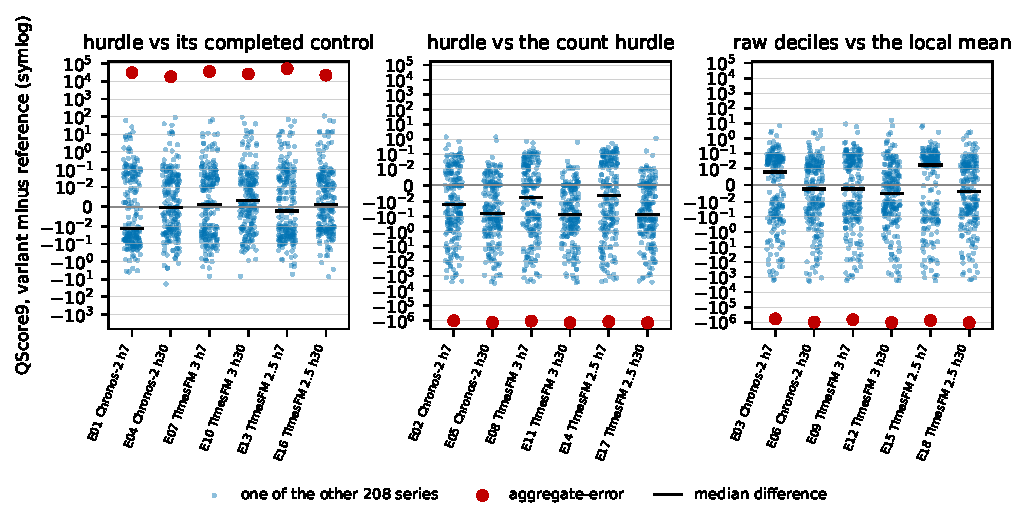
\includegraphics[width=\textwidth]{fig-s2-npm-paired-differences}
\caption{The eighteen external comparisons, series by series. Each point is one of the 209 series' paired
difference (variant minus reference \qs{}, three origins averaged) on a symmetric log scale, grouped by
contrast; the filled red marker is \texttt{aggregate-error}, and the short bar is the median. The mean of
each row, in Table~\ref{tab:s2ext}, is the red marker's value divided by 209 plus a remainder of a different
order.}
\label{fig:s2npm}
\end{figure}

\begin{table}[htbp]
\centering\small
\caption{The hurdle-minus-control difference (E01, E04, E07, E10, E13, E16 on npm; S01, S03, S05 on the
grid) and its three exact accounting parts, each divided by the full horizon: the loss on zero target days,
the loss on positive days from quantiles above the target (overprediction) and from quantiles below it
(underprediction). Equal-series and equal-block means; the parts sum to the total. Negative favors the
hurdle. The npm parts are unscaled and \texttt{aggregate-error} dominates them.}
\label{tab:s2parts}
\begin{tabular}{llrrrrr}
\toprule
Study & Model & $h$ & Total & Zero days & Positive, overprediction & Positive, underprediction \\
\midrule
npm & Chronos-2 & 7 & 152 & -0.3176 & -161.7 & 314 \\
npm & TimesFM 3 & 7 & 176.9 & -0.3701 & -149.5 & 326.8 \\
npm & TimesFM 2.5 & 7 & 253.9 & -0.3425 & -91.81 & 346 \\
npm & Chronos-2 & 30 & 90.24 & -63.79 & -146.1 & 300.1 \\
npm & TimesFM 3 & 30 & 128.5 & -66.08 & -112.9 & 307.5 \\
npm & TimesFM 2.5 & 30 & 110.3 & -67.09 & -131.9 & 309.4 \\
synthetic & Chronos-2 & 30 & 0.08599 & -0.1752 & -0.03194 & 0.2931 \\
synthetic & TimesFM 3 & 30 & 0.08662 & -0.172 & -0.0282 & 0.2868 \\
synthetic & TimesFM 2.5 & 30 & 0.08769 & -0.2293 & -0.03873 & 0.3557 \\
\bottomrule
\end{tabular}
\end{table}

\paragraph{By stratum.} The strata are declared secondary descriptors and carry no interval and no test;
the very sparse stratum holds $n = 9$ series, not 100. Against its completed control the hurdle variant
scores lower on 32 to 43 of the 100 dense series across the six cells, on 45 to 81 of the 100 sparse
series, and on 2 to 4 of the 9 very sparse series, where the median difference is exactly 0 in five of the
six cells. Against \hc{} it scores lower on 80 to 94 of the 100 dense series, on 29 to 63 of the 100 sparse
series and on 4 of the 9 very sparse series in every cell, with a median of exactly 0 there in all six. The
raw deciles score lower than \lm{} on 61 to 70 dense, 19 to 51 sparse and 4 or 5 very sparse series. With
nine series the very sparse stratum supports no reading beyond those counts (Table~\ref{tab:s2strata}).
Table~\ref{tab:s2regime} adds, post hoc and with no registered status, the lower-tied-higher counts, the
median and a raw two-sided signed-rank $p$ for the hurdle against its control within each stratum, computed
from the saved per-series scores; Table~\ref{tab:s2empirical} does the same for the hurdle against the
registered secondary \texttt{hurdle\_empirical\_28} by stratum and for the completed control against it
over all 209 series. A signed-rank test restricted to each stratum, computed post hoc from the saved per-series scores and
adding no registered test (Table~\ref{tab:s2regime}), has raw $p$ below 0.002 for all three
sparse-stratum contrasts at horizon 7 and from 0.47 to 0.892 at horizon 30. On the grid, by zero
probability, the hurdle beats its control in 4 to 6 of 30 replicate blocks at $z = 0.2$, in 12 to 15 at
$z = 0.8$ and in 21 to 26 at $z = 0.95$ (Table~\ref{tab:s2cells}). The dense result has a mechanical
cause: a series with no zero in its last 28 context days gets $p = 28.5 / 29$, so the hurdle forces about
1.7 percent of mass onto zero on every day, where the model's own completed law, which puts less there,
must win.

\begin{table}[htbp]
\centering\scriptsize\setlength{\tabcolsep}{2.4pt}
\caption{Post-hoc. The hurdle variant against its completed control within each stratum: ``L / T / H'', the
series where the hurdle is lower, tied or higher; the median difference; and the raw two-sided signed-rank
$p$ with zero differences omitted, computed from the saved per-series scores; no adjustment, no registered
status. The very sparse stratum holds $n = 9$.}
\label{tab:s2regime}
\begin{tabular}{llcrlcrlcrl}
\toprule
 & & \multicolumn{3}{c}{dense, $n = 100$} & \multicolumn{3}{c}{sparse, $n = 100$} & \multicolumn{3}{c}{very sparse, $n = 9$} \\
\cmidrule(lr){3-5} \cmidrule(lr){6-8} \cmidrule(lr){9-11}
Model & $h$ & L / T / H & Median & Raw $p$ & L / T / H & Median & Raw $p$ & L / T / H & Median & Raw $p$ \\
\midrule
Chronos-2 & 7 & 36 / 0 / 64 & 0.0455 & 0.0055 & 81 / 1 / 18 & -0.03333 & $2.47 \times 10^{-11}$ & 4 / 1 / 4 & 0 & 0.297 \\
TimesFM 3 & 7 & 32 / 0 / 68 & 0.03386 & 0.000363 & 60 / 3 / 37 & -0.009524 & 0.00158 & 2 / 5 / 2 & 0 & 0.625 \\
TimesFM 2.5 & 7 & 40 / 0 / 60 & 0.03386 & 0.00241 & 66 / 2 / 32 & -0.01058 & $9.01 \times 10^{-5}$ & 3 / 1 / 5 & 0.007407 & 0.82 \\
Chronos-2 & 30 & 43 / 0 / 57 & 0.01543 & 0.144 & 58 / 1 / 41 & -0.003086 & 0.47 & 4 / 1 / 4 & 0 & 0.312 \\
TimesFM 3 & 30 & 34 / 0 / 66 & 0.02173 & 0.000636 & 45 / 4 / 51 & 0.0004938 & 0.65 & 2 / 4 / 3 & 0 & 0.438 \\
TimesFM 2.5 & 30 & 43 / 0 / 57 & 0.02333 & 0.00106 & 54 / 0 / 46 & -0.0008642 & 0.892 & 4 / 1 / 4 & 0 & 0.312 \\
\bottomrule
\end{tabular}
\end{table}

\begin{table}[htbp]
\centering\footnotesize\setlength{\tabcolsep}{3.5pt}
\caption{Post-hoc. The foundation-model hurdle against the registered secondary
\texttt{hurdle\_empirical\_28}, which shares its occurrence rule and uses the empirical positive law, by
stratum (series where the hurdle is lower, tied or higher); and the completed control against the same
empirical hurdle over all 209 series, with the median difference and the raw two-sided signed-rank $p$.
Computed from the saved per-series scores; no adjustment, no registered status.}
\label{tab:s2empirical}
\begin{tabular}{llcccccl}
\toprule
 & & \multicolumn{3}{c}{hurdle vs empirical hurdle, lower / tied / higher} & \multicolumn{3}{c}{completed vs empirical hurdle, $n = 209$} \\
\cmidrule(lr){3-5} \cmidrule(lr){6-8}
Model & $h$ & dense, $n = 100$ & sparse, $n = 100$ & very sparse, $n = 9$ & Lower / tied / higher & Median & Raw $p$ \\
\midrule
Chronos-2 & 7 & 65 / 0 / 35 & 50 / 8 / 42 & 4 / 4 / 1 & 88 / 2 / 119 & 0.01058 & 0.598 \\
TimesFM 3 & 7 & 64 / 1 / 35 & 45 / 10 / 45 & 4 / 4 / 1 & 117 / 5 / 87 & -0.006349 & 0.00804 \\
TimesFM 2.5 & 7 & 63 / 0 / 37 & 33 / 3 / 64 & 4 / 4 / 1 & 90 / 1 / 118 & 0.009524 & 0.478 \\
Chronos-2 & 30 & 66 / 0 / 34 & 45 / 4 / 51 & 6 / 3 / 0 & 120 / 3 / 86 & -0.00716 & $4.94 \times 10^{-5}$ \\
TimesFM 3 & 30 & 68 / 0 / 32 & 55 / 13 / 32 & 5 / 4 / 0 & 140 / 8 / 61 & -0.01037 & $1.22 \times 10^{-8}$ \\
TimesFM 2.5 & 30 & 72 / 1 / 27 & 57 / 4 / 39 & 5 / 4 / 0 & 130 / 1 / 78 & -0.01012 & $5.1 \times 10^{-7}$ \\
\bottomrule
\end{tabular}
\end{table}

\begin{table}[htbp]
\centering\footnotesize\setlength{\tabcolsep}{3.5pt}
\caption{The context-scaled \qs{}, the registered scale-free secondary: each window's \qs{} divided by
$\max(1, \bar{y}_{\text{context}})$ before the registered averaging. Mean difference with its pointwise 95
percent bootstrap interval, median difference, and ``L / T / H'', the series (of 209) or blocks (of 30)
where the variant is lower, tied or higher. The synthetic rows are at horizon 30; the suffix \texttt{-h7}
marks the horizon-7 secondary rows.}
\label{tab:s2scaled}
\begin{tabular}{lllrrcrc}
\toprule
ID & Variant & Reference & $h$ & Mean & 95\% interval & Median & L / T / H \\
\midrule
E01 & chronos2\_hurdle & chronos2\_completed & 7 & -0.02204 & [-0.03098, -0.01407] & -0.005825 & 122 / 2 / 85 \\
E04 & chronos2\_hurdle & chronos2\_completed & 30 & -0.002395 & [-0.006836, 0.00146] & 0.0002262 & 101 / 2 / 106 \\
E02 & chronos2\_hurdle & hurdle\_count\_28 & 7 & -0.1311 & [-0.1809, -0.08701] & -0.01058 & 129 / 12 / 68 \\
E05 & chronos2\_hurdle & hurdle\_count\_28 & 30 & -0.1456 & [-0.1909, -0.1055] & -0.02617 & 150 / 9 / 50 \\
E03 & chronos2\_raw & local\_mean\_28 & 7 & -0.01511 & [-0.03735, 0.004919] & 0.003944 & 92 / 0 / 117 \\
E06 & chronos2\_raw & local\_mean\_28 & 30 & -0.02913 & [-0.04976, -0.01305] & -0.00184 & 112 / 0 / 97 \\
E07 & timesfm3\_hurdle & timesfm3\_completed & 7 & -0.006708 & [-0.01467, -0.0001148] & 0.0008949 & 95 / 8 / 106 \\
E10 & timesfm3\_hurdle & timesfm3\_completed & 30 & 0.001291 & [-0.001255, 0.003757] & 0.001769 & 80 / 8 / 121 \\
E08 & timesfm3\_hurdle & hurdle\_count\_28 & 7 & -0.1278 & [-0.1761, -0.08451] & -0.004233 & 116 / 18 / 75 \\
E11 & timesfm3\_hurdle & hurdle\_count\_28 & 30 & -0.1466 & [-0.19, -0.1075] & -0.03038 & 161 / 17 / 31 \\
E09 & timesfm3\_raw & local\_mean\_28 & 7 & -0.02463 & [-0.04487, -0.007124] & -0.001849 & 112 / 1 / 96 \\
E12 & timesfm3\_raw & local\_mean\_28 & 30 & -0.03336 & [-0.05248, -0.01843] & -0.003988 & 124 / 1 / 84 \\
E13 & timesfm2p5\_hurdle & timesfm2p5\_completed & 7 & -0.006123 & [-0.01111, -0.001495] & -0.001063 & 110 / 2 / 97 \\
E16 & timesfm2p5\_hurdle & timesfm2p5\_completed & 30 & 0.001687 & [-0.0008144, 0.004384] & 0.0006744 & 101 / 1 / 107 \\
E14 & timesfm2p5\_hurdle & hurdle\_count\_28 & 7 & -0.1182 & [-0.1673, -0.07431] & -0.004233 & 113 / 7 / 89 \\
E17 & timesfm2p5\_hurdle & hurdle\_count\_28 & 30 & -0.1402 & [-0.1839, -0.1025] & -0.02686 & 160 / 9 / 40 \\
E15 & timesfm2p5\_raw & local\_mean\_28 & 7 & -0.01512 & [-0.03593, 0.001938] & 0.008833 & 82 / 1 / 126 \\
E18 & timesfm2p5\_raw & local\_mean\_28 & 30 & -0.02597 & [-0.04489, -0.01163] & -0.00242 & 109 / 1 / 99 \\
\midrule
S01-h7 & chronos2\_hurdle & chronos2\_completed & 7 & 0.03751 & [0.01416, 0.06281] & 0.01705 & 8 / 0 / 22 \\
S01 & chronos2\_hurdle & chronos2\_completed & 30 & 0.00139 & [-0.01216, 0.01501] & 0.004498 & 14 / 0 / 16 \\
S02-h7 & chronos2\_hurdle & hurdle\_count\_28 & 7 & 0.001251 & [-0.01012, 0.01276] & 0.00345 & 13 / 0 / 17 \\
S02 & chronos2\_hurdle & hurdle\_count\_28 & 30 & -0.0003784 & [-0.007165, 0.006157] & 0.002033 & 13 / 0 / 17 \\
S03-h7 & timesfm3\_hurdle & timesfm3\_completed & 7 & 0.0397 & [0.01707, 0.06452] & 0.0193 & 8 / 0 / 22 \\
S03 & timesfm3\_hurdle & timesfm3\_completed & 30 & 0.007152 & [-0.00766, 0.02042] & 0.006261 & 10 / 0 / 20 \\
S04-h7 & timesfm3\_hurdle & hurdle\_count\_28 & 7 & -0.001183 & [-0.01205, 0.009608] & 0.0006988 & 15 / 0 / 15 \\
S04 & timesfm3\_hurdle & hurdle\_count\_28 & 30 & -0.003914 & [-0.01056, 0.001931] & 0.001094 & 14 / 0 / 16 \\
S05-h7 & timesfm2p5\_hurdle & timesfm2p5\_completed & 7 & 0.03654 & [0.01467, 0.06046] & 0.02256 & 7 / 0 / 23 \\
S05 & timesfm2p5\_hurdle & timesfm2p5\_completed & 30 & 0.006541 & [-0.007033, 0.01877] & 0.006349 & 12 / 0 / 18 \\
S06-h7 & timesfm2p5\_hurdle & hurdle\_count\_28 & 7 & 0.003006 & [-0.009649, 0.01578] & 0.002948 & 13 / 0 / 17 \\
S06 & timesfm2p5\_hurdle & hurdle\_count\_28 & 30 & 0.0004433 & [-0.008125, 0.008421] & 0.002583 & 12 / 0 / 18 \\
\bottomrule
\end{tabular}
\end{table}

\begin{table}[htbp]
\centering\footnotesize\setlength{\tabcolsep}{3.5pt}
\caption{The eighteen external comparisons by context-zero-fraction stratum, declared secondary, with no
interval and no test: the mean difference, the median difference and the number of series where the variant
is lower, for the dense ($n = 100$), sparse ($n = 100$) and very sparse ($n = 9$) strata. The dense means
are unscaled and carried by \texttt{aggregate-error}.}
\label{tab:s2strata}
\begin{tabular}{lrrrrrrrrr}
\toprule
 & \multicolumn{3}{c}{dense, $n = 100$} & \multicolumn{3}{c}{sparse, $n = 100$} & \multicolumn{3}{c}{very sparse, $n = 9$} \\
\cmidrule(lr){2-4} \cmidrule(lr){5-7} \cmidrule(lr){8-10}
ID & Mean & Median & Lower & Mean & Median & Lower & Mean & Median & Lower \\
\midrule
E01 & 317.7 & 0.0455 & 36 & -0.05531 & -0.03333 & 81 & -0.01752 & 0 & 4 \\
E02 & -10,638 & -0.3217 & 85 & -0.3483 & 0.003175 & 40 & -1.312 & 0 & 4 \\
E03 & -6,028 & -0.07942 & 62 & -0.001134 & 0.0266 & 26 & 0.0684 & $1.055 \times 10^{-9}$ & 4 \\
E04 & 188.6 & 0.01543 & 43 & -0.01457 & -0.003086 & 58 & -0.01108 & 0 & 4 \\
E05 & -13,715 & -0.6031 & 91 & -0.3834 & -0.001728 & 55 & -1.415 & 0 & 4 \\
E06 & -9,893 & -0.03933 & 61 & -0.04493 & 0.00175 & 46 & -0.006479 & -0.006837 & 5 \\
E07 & 369.7 & 0.03386 & 32 & -0.03119 & -0.009524 & 60 & 0.01129 & 0 & 2 \\
E08 & -11,318 & -0.3767 & 80 & -0.3252 & 0.003175 & 32 & -1.307 & 0 & 4 \\
E09 & -6,761 & -0.1083 & 70 & 0.002103 & 0.01057 & 38 & 0.04384 & 0 & 4 \\
E10 & 268.6 & 0.02173 & 34 & -0.0003926 & 0.0004938 & 45 & 0.02148 & 0 & 2 \\
E11 & -14,194 & -0.5769 & 94 & -0.3521 & -0.004444 & 63 & -1.39 & 0 & 4 \\
E12 & -10,452 & -0.04297 & 70 & -0.02674 & -0.0006202 & 51 & -0.0149 & 0 & 4 \\
E13 & 530.6 & 0.03386 & 40 & -0.01284 & -0.01058 & 66 & -0.003645 & 0.007407 & 3 \\
E14 & -12,220 & -0.3709 & 82 & -0.3162 & 0.01323 & 29 & -1.31 & 0 & 4 \\
E15 & -7,823 & -0.1053 & 61 & -0.005074 & 0.03205 & 19 & 0.05747 & 0 & 4 \\
E16 & 230.6 & 0.02333 & 43 & 0.01899 & -0.0008642 & 54 & -0.003841 & 0 & 4 \\
E17 & -14,458 & -0.5962 & 94 & -0.3428 & -0.003086 & 62 & -1.409 & 0 & 4 \\
E18 & -10,678 & -0.05805 & 68 & -0.03236 & 0.004494 & 40 & -0.006367 & -0.003695 & 5 \\
\bottomrule
\end{tabular}
\end{table}

\paragraph{The three zero days, the counts.} After the run was scored, the saved targets were found to
read 0 for every one of the 209 series on 2026-07-12 and 2026-08-14, and 0 for \texttt{aggregate-error}
alone on 2026-06-25, between days of millions. The registered completeness rule, fixed before any target was
seen, does not test for a source-wide zero, so the three days were scored as served; each falls in one
horizon-30 block and in no horizon-7 block. The dated addition of 2026-10-16 to the protocol, item 6, made
after the scores were seen, keeps the registered analysis of the data as served as the confirmatory result
for E01 to E18 and asks that a post-hoc sensitivity which removes the days be reported beside it; that
sensitivity, computed at 03:21 UTC on 2026-10-16 before the addition was written at 03:28 UTC and committed
with it, is below. On 2026-07-12 and 2026-08-14 the panel's total is 0
between neighbours of 4,059,870 and 10,123,968 downloads, and 7,480,108 and 2,560,140; on 2026-06-25
\texttt{aggregate-error} reads 0 between 9,475,033 and 7,909,626, when 92 of the 209 series read 0 against
98 and 121 on the days either side. No day of the 275-day context reads 0 for more than 153 of the 209
series, and the largest series never reads below 1,109,682 there. npm's own status history, trackers and
changelog report no outage, gap or backfill for the three days, and the status page does not track download
counts. In the post-hoc sensitivity of Table~\ref{tab:s2sens} each removed day is dropped, for every series
and variant, from the one horizon-30 block that holds it; the horizon-7 blocks hold none of the days and
their rows are identical except for their adjusted $p$, which moves because the adjustment ranks all
eighteen together; the same code reproduces the registered tables byte for byte on the saved scores. The day
that touches only the largest series, 2026-06-25, differs in kind from the two panel-wide days only in its
reach; the sensitivity treats all three alike. Each removed day is dropped from the one horizon-30 block that
holds it, the block is re-scored over its remaining 29 days, and the registered aggregation, test, seeded
bootstrap and one adjustment run unchanged. Without all three days, which re-scores 10,032 forecasts, none
of the eighteen conclusions changes: no row changes the side with the larger signed-rank sum, the sign of
its mean or its rejection. Without the two panel-wide days only, which re-scores 6,688 forecasts, one
conclusion changes: E06, Chronos-2's raw deciles against \lm{} at horizon 30, no longer rejects, with
adjusted $p$ 0.0599 and raw $p$ 0.0399 against 0.0119 and 0.00663 registered; it still favors the model by
rank sum, with the model lower on 110 of 209 series. Without the three days the hurdle-against-control means
at horizon 30 grow, E04 from 90.24 to 159.3, E10 from 128.5 to 201.2 and E16 from 110.3 to 183.4, and those
means belong to \texttt{aggregate-error}. The mechanism answer does not depend on the three days.

\begin{table}[htbp]
\centering\footnotesize\setlength{\tabcolsep}{3.5pt}
\caption{Post-hoc. The eighteen external comparisons as registered and under the two removals of the npm
zero days: the mean difference, the adjusted $p$ and whether the test rejects at $q = 0.05$ after one
adjustment over the eighteen of each scenario; the last column is the side with the larger signed-rank sum,
the same in all three analyses. The horizon-7 rows are unchanged except for their adjusted $p$. The means
are unscaled and carried by \texttt{aggregate-error}.}
\label{tab:s2sens}
\begin{tabular}{lrllrllrlll}
\toprule
 & \multicolumn{3}{c}{Registered} & \multicolumn{3}{c}{Without the three days} & \multicolumn{3}{c}{Without the two panel-wide days} & \\
\cmidrule(lr){2-4} \cmidrule(lr){5-7} \cmidrule(lr){8-10}
ID & Mean & Adj.\ $p$ & Rejects & Mean & Adj.\ $p$ & Rejects & Mean & Adj.\ $p$ & Rejects & Favors \\
\midrule
E01 & 152 & 0.203 & no & 152 & 0.188 & no & 152 & 0.203 & no & model \\
E02 & -5,090 & $3.72 \times 10^{-11}$ & yes & -5,090 & $3.72 \times 10^{-11}$ & yes & -5,090 & $3.72 \times 10^{-11}$ & yes & model \\
E03 & -2,884 & 0.596 & no & -2,884 & 0.596 & no & -2,884 & 0.596 & no & model \\
E04 & 90.24 & 0.449 & no & 159.3 & 0.188 & no & 143.4 & 0.23 & no & reference \\
E05 & -6,563 & $7.06 \times 10^{-21}$ & yes & -6,473 & $2.89 \times 10^{-20}$ & yes & -6,311 & $3.76 \times 10^{-20}$ & yes & model \\
E06 & -4,734 & 0.0119 & yes & -4,834 & 0.0359 & yes & -4,646 & 0.0599 & no & model \\
E07 & 176.9 & 0.236 & no & 176.9 & 0.22 & no & 176.9 & 0.23 & no & reference \\
E08 & -5,416 & $3.61 \times 10^{-8}$ & yes & -5,416 & $3.61 \times 10^{-8}$ & yes & -5,416 & $3.61 \times 10^{-8}$ & yes & model \\
E09 & -3,235 & 0.0438 & yes & -3,235 & 0.0438 & yes & -3,235 & 0.0478 & yes & model \\
E10 & 128.5 & 0.00215 & yes & 201.2 & 0.00179 & yes & 184.9 & 0.00211 & yes & reference \\
E11 & -6,792 & $3.19 \times 10^{-25}$ & yes & -6,744 & $2.33 \times 10^{-24}$ & yes & -6,563 & $1.16 \times 10^{-24}$ & yes & model \\
E12 & -5,001 & $3.82 \times 10^{-5}$ & yes & -5,147 & $5.84 \times 10^{-5}$ & yes & -4,940 & $8.76 \times 10^{-5}$ & yes & model \\
E13 & 253.9 & 0.628 & no & 253.9 & 0.628 & no & 253.9 & 0.628 & no & reference \\
E14 & -5,847 & $2.66 \times 10^{-5}$ & yes & -5,847 & $2.66 \times 10^{-5}$ & yes & -5,847 & $2.66 \times 10^{-5}$ & yes & model \\
E15 & -3,743 & 0.746 & no & -3,743 & 0.746 & no & -3,743 & 0.746 & no & model \\
E16 & 110.3 & 0.0276 & yes & 183.4 & 0.0257 & yes & 167.1 & 0.0344 & yes & reference \\
E17 & -6,918 & $1.77 \times 10^{-23}$ & yes & -6,857 & $4.79 \times 10^{-22}$ & yes & -6,709 & $2.46 \times 10^{-22}$ & yes & model \\
E18 & -5,109 & 0.00204 & yes & -5,242 & 0.00988 & yes & -5,068 & 0.00638 & yes & model \\
\bottomrule
\end{tabular}
\end{table}

\begin{table}[htbp]
\centering\footnotesize\setlength{\tabcolsep}{3.5pt}
\caption{The six synthetic comparisons cell by cell at horizon 30: the mean paired difference over the 30
replicates of each cell and, in brackets, the replicates where the hurdle variant is lower; no interval and
no test. Under the declared rule only an exact zero is a tie, and a difference of order $10^{-18}$ is
floating-point residue. In the cells with $\mu_{+} = 1$ the positive law is degenerate at one.}
\label{tab:s2cells}
\begin{tabular}{lrrrcccccc}
\toprule
Cell & $z$ & $\mu_{+}$ & $\rho$ & S01 & S02 & S03 & S04 & S05 & S06 \\
\midrule
cell00 & 0.2 & 1 & 0.0 & 0.001276 (10) & 0 (0) & -0.0008477 (9) & 0 (0) & $1.85 \times 10^{-18}$ (16) & 0 (0) \\
cell01 & 0.2 & 1 & 0.8 & 0.02091 (11) & 0.004074 (0) & 0.0309 (9) & 0.00177 (0) & 0.0307 (12) & 0.001786 (0) \\
cell02 & 0.2 & 5 & 0.0 & 0.03719 (7) & 0.03202 (6) & 0.02129 (6) & 0.007078 (14) & 0.02285 (8) & 0.01269 (12) \\
cell03 & 0.2 & 5 & 0.8 & 0.1172 (11) & 0.03621 (11) & 0.127 (9) & 0.02497 (9) & 0.166 (8) & 0.03737 (9) \\
cell04 & 0.2 & 25 & 0.0 & 0.4659 (1) & 0.5156 (0) & 0.3406 (2) & 0.3273 (0) & 0.4349 (3) & 0.5687 (0) \\
cell05 & 0.2 & 25 & 0.8 & 0.9766 (8) & 0.5322 (8) & 0.9342 (7) & 0.3082 (9) & 0.969 (7) & 0.5615 (7) \\
cell06 & 0.8 & 1 & 0.0 & 0.003021 (9) & 0.002947 (0) & 0.001531 (6) & 0 (0) & -0.002148 (16) & 0.0002058 (0) \\
cell07 & 0.8 & 1 & 0.8 & 0.01146 (12) & 0.003679 (0) & 0.02715 (13) & 0.002634 (0) & 0.02033 (11) & 0.004247 (0) \\
cell08 & 0.8 & 5 & 0.0 & 0.005045 (11) & 0.0007407 (15) & -0.002477 (14) & 0.0001235 (11) & -0.005309 (16) & 0.01626 (8) \\
cell09 & 0.8 & 5 & 0.8 & 0.01672 (17) & -0.01305 (17) & 0.05014 (14) & -0.01853 (18) & 0.02598 (15) & -0.0224 (17) \\
cell10 & 0.8 & 25 & 0.0 & 0.08187 (6) & 0.09585 (8) & 0.04629 (10) & 0.05008 (10) & -0.02146 (15) & 0.1869 (6) \\
cell11 & 0.8 & 25 & 0.8 & 0.1006 (20) & -0.1548 (17) & 0.2028 (18) & -0.2022 (18) & 0.1279 (15) & -0.1151 (17) \\
cell12 & 0.95 & 1 & 0.0 & 0.001374 (1) & 0 (0) & -0.0002305 (12) & 0 (0) & 0.001481 (1) & 0 (0) \\
cell13 & 0.95 & 1 & 0.8 & -0.006831 (8) & 0.0003951 (0) & 0.001753 (7) & 0.0005844 (0) & 0.004247 (3) & 0.0005514 (0) \\
cell14 & 0.95 & 5 & 0.0 & 0.0002551 (5) & -0.004444 (9) & -0.006988 (23) & -0.003564 (9) & -0.0008971 (10) & -0.004444 (9) \\
cell15 & 0.95 & 5 & 0.8 & -0.04295 (13) & -0.005226 (9) & -0.02037 (9) & -0.01003 (9) & -0.01931 (5) & -0.01541 (9) \\
cell16 & 0.95 & 25 & 0.0 & -0.005218 (24) & -0.03199 (8) & -0.04486 (28) & -0.02057 (8) & -0.02882 (28) & -0.03235 (8) \\
cell17 & 0.95 & 25 & 0.8 & -0.2365 (15) & -0.07619 (9) & -0.1487 (13) & -0.08094 (9) & -0.147 (12) & -0.101 (9) \\
\bottomrule
\end{tabular}
\end{table}

\paragraph{The context-scaled score.} The registered scale-free secondary, which divides each window's \qs{}
by the context mean before the same averaging, reads differently from the unscaled mean on the hurdle
contrast (Table~\ref{tab:s2scaled}). At horizon 7 the scaled difference against the completed
control favors the hurdle for all three models, -0.02204 for Chronos-2, -0.006708 for TimesFM 3 and
-0.006123 for TimesFM 2.5, with every interval below zero; at horizon 30 every interval includes zero
(-0.002395, 0.001291 and 0.001687). Against \hc{} the scaled differences are -0.1182 to -0.1466 with every
interval below zero, and against \lm{} they are below zero in the four cells that reject (E06, E09, E12,
E18) and include zero in E03 and E15. On the grid every scaled interval includes zero at horizon 30; the
largest unscaled cell differences are in the cells with $z = 0.2$ and $\mu_{+} = 25$, which scaling by the
context mean weighs least. The occurrence Brier score, available where a count law exists, is lower for the
hurdle than for its control with an interval below zero in E01, E04 and E13 and includes zero in E07, E10
and E16; on the mean the models' own zero mass is about as good as the Jeffreys estimate
(Tables~\ref{tab:s2scores} and~\ref{tab:s2synscores}). These are secondary readings and add no test.

\begin{table}[htbp]
\centering\footnotesize\setlength{\tabcolsep}{3.5pt}
\caption{Mean scores of the sixteen variants on the npm panel (209 series, equal weights): \qs{} at both
horizons and, at horizon 30, the context-scaled \qs{}, the occurrence Brier score and the discrete CRPS
where a count law exists. The CRPS is over 208 series, \texttt{aggregate-error} being unavailable. The
unscaled means are carried by \texttt{aggregate-error}, except the horizon-30 mean of \aets{}, which one
other series, \texttt{composer-runtime-pouchdb}, carries; it is in no family comparison.}
\label{tab:s2scores}
\begin{tabular}{lrrrrr}
\toprule
Variant & \qs{} $h = 7$ & \qs{} $h = 30$ & Scaled \qs{} $h = 30$ & Brier $h = 30$ & CRPS $h = 30$ \\
\midrule
chronos2\_raw & 4,500 & 4,226 & 0.9315 &  &  \\
chronos2\_completed & 4,500 & 4,226 & 0.9283 & 0.1817 & 57.61 \\
chronos2\_hurdle & 4,652 & 4,316 & 0.9259 & 0.1785 & 58.27 \\
timesfm3\_raw & 4,149 & 3,958 & 0.9273 &  &  \\
timesfm3\_completed & 4,149 & 3,958 & 0.9236 & 0.179 & 56.22 \\
timesfm3\_hurdle & 4,326 & 4,087 & 0.9249 & 0.1785 & 57.15 \\
timesfm2p5\_raw & 3,641 & 3,850 & 0.9347 &  &  \\
timesfm2p5\_completed & 3,641 & 3,850 & 0.9296 & 0.1795 & 59.72 \\
timesfm2p5\_hurdle & 3,895 & 3,960 & 0.9313 & 0.1785 & 61.02 \\
local\_mean\_28 & 7,384 & 8,959 & 0.9607 &  &  \\
autoets\_weekly & 4,756 & 74,699 & 291.8 &  &  \\
nb\_local\_level\_28 & 7,741 & 8,739 & 0.9801 & 0.2117 & 99.49 \\
poisson\_28 & 9,630 & 10,642 & 1.132 & 0.2291 & 123.6 \\
hurdle\_count\_28 & 9,742 & 10,878 & 1.072 & 0.1785 & 118.5 \\
hurdle\_empirical\_28 & 7,348 & 8,685 & 0.9565 & 0.1785 & 88.76 \\
dynamic\_count & 10,948 & 11,471 & 1.026 & 0.1773 & 124.2 \\
\bottomrule
\end{tabular}
\end{table}

\begin{table}[htbp]
\centering\footnotesize\setlength{\tabcolsep}{3.5pt}
\caption{Mean scores of the sixteen variants and the oracle on the synthetic grid (30 replicate blocks,
18 cells with equal weight): \qs{} at both horizons and, at horizon 30, the occurrence Brier score and the
discrete CRPS where a count law exists. The oracle is a diagnostic, not a competitor;
\texttt{dynamic\_count} has the lowest \qs{} of the sixteen variants at horizon 30.}
\label{tab:s2synscores}
\begin{tabular}{lrrrr}
\toprule
Variant & \qs{} $h = 7$ & \qs{} $h = 30$ & Brier $h = 30$ & CRPS $h = 30$ \\
\midrule
chronos2\_raw & 1.613 & 1.791 &  &  \\
chronos2\_completed & 1.607 & 1.785 & 0.1329 & 1.653 \\
chronos2\_hurdle & 1.805 & 1.871 & 0.1325 & 1.728 \\
timesfm3\_raw & 1.594 & 1.758 &  &  \\
timesfm3\_completed & 1.589 & 1.754 & 0.1299 & 1.619 \\
timesfm3\_hurdle & 1.783 & 1.84 & 0.1325 & 1.695 \\
timesfm2p5\_raw & 1.638 & 1.8 &  &  \\
timesfm2p5\_completed & 1.63 & 1.792 & 0.1366 & 1.656 \\
timesfm2p5\_hurdle & 1.818 & 1.88 & 0.1325 & 1.74 \\
local\_mean\_28 & 1.762 & 1.836 &  &  \\
autoets\_weekly & 1.884 & 2.211 &  &  \\
nb\_local\_level\_28 & 1.855 & 1.911 & 0.1475 & 1.773 \\
poisson\_28 & 2.16 & 2.255 & 0.2417 & 2.14 \\
hurdle\_count\_28 & 1.739 & 1.819 & 0.1325 & 1.677 \\
hurdle\_empirical\_28 & 1.747 & 1.825 & 0.1325 & 1.685 \\
dynamic\_count & 1.632 & 1.721 & 0.1236 & 1.588 \\
oracle & 1.514 & 1.648 & 0.115 & 1.504 \\
\bottomrule
\end{tabular}
\end{table}

\paragraph{The oracle, as a diagnostic.} The oracle that knows the generator's parameters and the last
observed state has the lowest mean \qs{} of the seventeen forecasters at both horizons (1.514 at horizon 7
and 1.648 at horizon 30), the lowest occurrence Brier score (0.115) and the lowest discrete CRPS (1.504) at
horizon 30, and no forecaster scores below it in 17 of the 18 cells at horizon 30; in three of them
(\texttt{cell12}, \texttt{cell14} and \texttt{cell16}, with $z = 0.95$ and $\rho = 0$) \texttt{dynamic\_count}
ties it exactly, and in the cell with $z = 0.2$, $\mu_{+} = 1$ and $\rho = 0$, two forecasters score slightly
below it (0.1759 and 0.1761 against 0.1767), as the protocol allows for a finite sample. Its randomized PIT
histogram is flat, each tenth holding 0.099 to 0.104 of its 48,600 target days, where the six
foundation-model variants and \hc{} place 0.078 to 0.133 of theirs in a tenth. On npm each hurdle variant
places 0.088 to 0.146 of its horizon-30 target days in a tenth, against 0.083 to 0.153 for its completed
control. The oracle is neither a competitor nor a confirmatory contrast.

\paragraph{Per cell.} Figure~\ref{fig:s2cells} and Table~\ref{tab:s2cells} give the six synthetic
contrasts cell by cell at horizon 30, each over 30 replicates, with no interval and no test. The largest
differences against the hurdle are in the cells with $z = 0.2$ and $\mu_{+} = 25$, where the hurdle scores
0.9342 to 0.9766 above its control at $\rho = 0.8$; in the four cells with $z = 0.95$ and $\mu_{+}$ of 5 or
25, 23 of the 24 differences are negative, favoring the hurdle, and all are small beside those. Over the six
cells with $z = 0.95$ at horizon 30, read post hoc from the per-series scores, the hurdle is lower than its
control in 21, 26 and 23 of the 30 replicate blocks under \qs{}, in 24, 24 and 22 under the occurrence Brier
score and in 25, 26 and 22 under the discrete CRPS, and over the 540 series pairs \qs{} ties exactly on 232
and favors the hurdle on 217 of the other 308; at horizon 7 the blocks split 10, 14 and 18 of 30 under
\qs{}. In the cells with $\mu_{+} = 1$ the positive law is degenerate at one, and against \hc{} the hurdle is
lower in none of the 30 replicates in any of those six cells.

\begin{figure}[htbp]
\centering
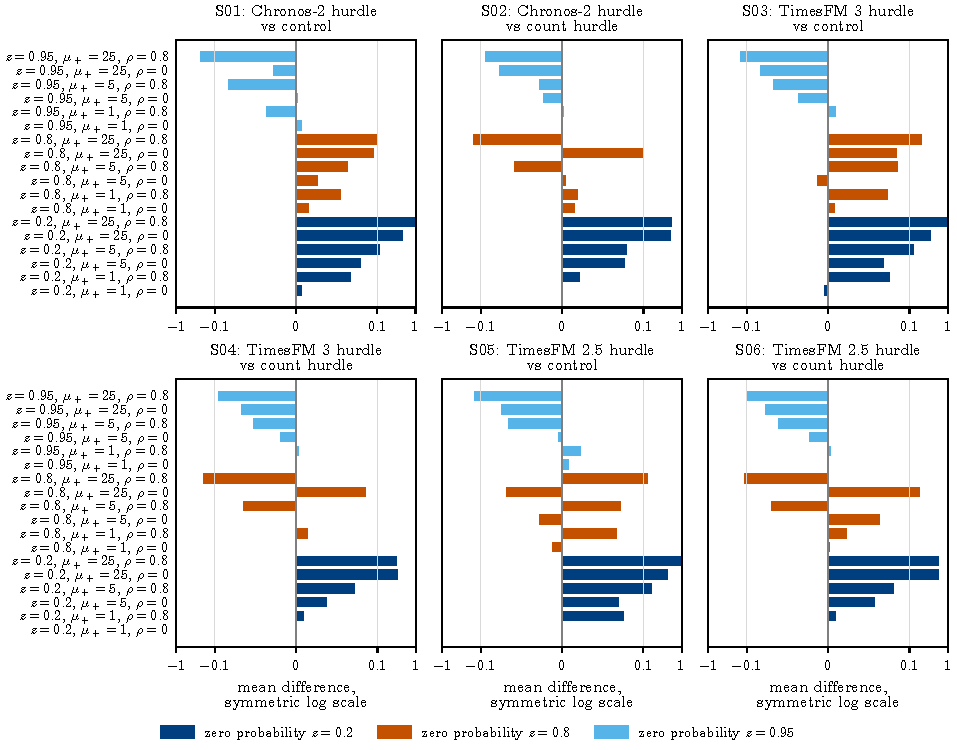
\includegraphics[width=\textwidth]{fig-s2-synthetic-cells}
\caption{The six synthetic comparisons, cell by cell at horizon 30: the mean paired difference over 30
replicates in each of the 18 generator cells, labeled by zero probability $z$, positive mean $\mu_{+}$ and
persistence $\rho$. Negative favors the hurdle variant. The family tests pool the cells with equal weight
(Table~\ref{tab:s2syn}); the cells carry no test.}
\label{fig:s2cells}
\end{figure}

\paragraph{The dynamic-occurrence post-hoc, the detail.} The analysis summarized in
Section~\ref{sec:discussion} is post-hoc. It was computed on 2026-10-16 from the saved forecasts of both
runs, after the registered scores were seen, with no registered status; it adds no test to E01 to E18 or
S01 to S06 and replaces nothing in them, and no model was run. The registered hurdle's occurrence estimate is constant over
the horizon and ignores persistence; the registered \texttt{dynamic\_count} baseline carries a dynamic one,
the discounted Beta-Bernoulli with discount 0.98. The wrapper tested here is the registered hurdle with the
Jeffreys $p$ replaced by $p_{\text{dyn}} = a_B / (a_B + b_B)$, read from \texttt{dynamic\_count}'s saved law
for the same day, with $G_+$ the model's saved completed positive law exactly as the registered hurdle uses
it; where \texttt{dynamic\_count} falls back to \hc{} by its registered rule, in 10 of the 627 npm windows
at each horizon and 501 of the 1,620 grid windows, the wrapper is the registered hurdle. Each wrapper is
compared with the model's completed control, the model's registered hurdle, \texttt{dynamic\_count} (whose
occurrence it shares on every day, so the positive law alone differs) and \hc{}: 24 tests on npm, DE01 to
DE24, and 12 on the grid, DS01 to DS12, each family with the registered settings and its own
Benjamini-Hochberg adjustment at $q = 0.05$. Before any output was written the command verified every
checkpoint hash, rebuilt both registered families byte for byte from the saved scores, and reproduced the
registered hurdle exactly in every window when given the Jeffreys $p$. Table~\ref{tab:s2dyn} gives the rows
against the completed control and the registered hurdle, and Table~\ref{tab:s2dynrest} the rows against
\texttt{dynamic\_count}, whose occurrence each wrapper shares on every day, and against \hc{};
Table~\ref{tab:s2dynparts} gives the three accounting parts of the wrappers and their references on the
grid at horizon 30, each an equal-block mean over the full horizon, and the parts sum to \qs{}.

\begin{table}[htbp]
\centering\footnotesize\setlength{\tabcolsep}{3.5pt}
\caption{Post-hoc. The model's completed positive law wrapped with \texttt{dynamic\_count}'s occurrence,
against the model's completed control and against the model's registered fixed-occurrence hurdle, on npm
(DE rows, 209 series) and the grid (DS rows, 30 replicate blocks at horizon 30). Differences are wrapper
minus reference \qs{}; negative favors the wrapper. The interval is the pointwise 95 percent percentile
interval from 20,000 entity bootstrap replicates; $p$ is Benjamini-Hochberg adjusted once over the 24 npm or
the 12 grid post-hoc tests. ``L / T / H'' counts the series or blocks where the wrapper is lower, tied or
higher. The npm means are unscaled and carried by \texttt{aggregate-error}; a median of order $10^{-17}$ is
floating-point residue.}
\label{tab:s2dyn}
\begin{tabular}{lllrrcrcl}
\toprule
ID & Model & Reference & $h$ & Mean & 95\% interval & Median & L / T / H & Adjusted $p$ \\
\midrule
DE01 & Chronos-2 & completed & 7 & 77.33 & [-0.008112, 231.6] & -0.009524 & 116 / 5 / 88 & 0.24 \\
DE04 & Chronos-2 & fixed hurdle & 7 & -74.67 & [-223.6, -0.148] & -0.001058 & 106 / 6 / 97 & 0.203 \\
DE05 & Chronos-2 & completed & 30 & 26.03 & [-0.05339, 77.77] & -0.005679 & 126 / 4 / 79 & 0.112 \\
DE08 & Chronos-2 & fixed hurdle & 30 & -64.21 & [-191.9, -0.2468] & -0.007901 & 138 / 3 / 68 & $1.64 \times 10^{-6}$ \\
DE09 & TimesFM 3 & completed & 7 & 93.25 & [-0.0469, 279.4] & 0.004233 & 80 / 15 / 114 & 0.121 \\
DE12 & TimesFM 3 & fixed hurdle & 7 & -83.65 & [-250.3, -0.2098] & 0 & 102 / 5 / 102 & 0.367 \\
DE13 & TimesFM 3 & completed & 30 & 54.04 & [-0.09206, 161.8] & -0.0002469 & 106 / 11 / 92 & 0.838 \\
DE16 & TimesFM 3 & fixed hurdle & 30 & -74.49 & [-222.2, -0.4329] & -0.004938 & 131 / 7 / 71 & $6.88 \times 10^{-6}$ \\
DE17 & TimesFM 2.5 & completed & 7 & 82.61 & [0.1723, 247] & 0.002116 & 95 / 6 / 108 & 0.0787 \\
DE20 & TimesFM 2.5 & fixed hurdle & 7 & -171.3 & [-513, -0.2688] & 0.002116 & 93 / 8 / 108 & 0.794 \\
DE21 & TimesFM 2.5 & completed & 30 & 28.84 & [0.08909, 85.83] & $-5.551 \times 10^{-17}$ & 105 / 3 / 101 & 0.471 \\
DE24 & TimesFM 2.5 & fixed hurdle & 30 & -81.49 & [-242.9, -0.5095] & -0.004198 & 124 / 5 / 80 & 0.000642 \\
\midrule
DS01 & Chronos-2 & completed & 30 & 0.0278 & [-0.008979, 0.06239] & 0.04308 & 10 / 0 / 20 & 0.0959 \\
DS04 & Chronos-2 & fixed hurdle & 30 & -0.05819 & [-0.09786, -0.02406] & -0.04727 & 21 / 0 / 9 & 0.00823 \\
DS05 & TimesFM 3 & completed & 30 & 0.02813 & [-0.01113, 0.0638] & 0.02883 & 10 / 0 / 20 & 0.0959 \\
DS08 & TimesFM 3 & fixed hurdle & 30 & -0.05849 & [-0.09728, -0.02412] & -0.04468 & 21 / 0 / 9 & 0.00823 \\
DS09 & TimesFM 2.5 & completed & 30 & 0.03462 & [-0.004804, 0.07104] & 0.04275 & 7 / 0 / 23 & 0.0439 \\
DS12 & TimesFM 2.5 & fixed hurdle & 30 & -0.05307 & [-0.0902, -0.02105] & -0.03688 & 20 / 0 / 10 & 0.00823 \\
\bottomrule
\end{tabular}
\end{table}

The dynamic occurrence shrinks the loss and removes four of the five rejections against the substitution,
and it still never beats the model's own zero mass at $q = 0.05$. Against the completed control no npm row
rejects, with adjusted $p$ from 0.0787 to 0.838, where the registered hurdle had two rejections against it;
every mean difference is still positive, 26.03 to 93.25 against 90.24 to 253.9 for the registered hurdle,
and by rank sum the typical series leans to the Chronos-2 wrapper at both horizons, lower on 116 and 126 of
209 series, and to the control for both TimesFM models. On the grid two of the three rows against the
control no longer reject (DS01 and DS05, adjusted $p$ 0.0959) and the third, TimesFM 2.5 (DS09, adjusted $p$
0.0439), still rejects against the wrapper; the means are 0.0278 to 0.03462 against 0.08599 to 0.08769
registered, and every interval now includes zero. Against the registered fixed-occurrence hurdle the wrapper
is better at horizon 30 everywhere: on npm all three models reject in its favor, lower on 124 to 138 of 209
series, and on the grid all three reject in its favor, lower in 20 or 21 of 30 blocks (adjusted $p$
0.00823); at horizon 7 on npm no row rejects. Against \texttt{dynamic\_count} itself all six npm rows reject
in the wrapper's favor and all three grid rows reject against it, \texttt{dynamic\_count} being lower in 26
to 28 of 30 blocks; against \hc{} all six npm rows reject in the wrapper's favor and on the grid none of the
three rejects, where the registered S02 and S06 rejected against the hurdle. The accounting (Appendix
Table~\ref{tab:s2dynparts}) says where the remaining loss sits: on the grid the wrapper has the lowest
zero-day part of every forecaster, 0.3653 to 0.3879, while its positive-day underprediction part stays at
1.303 to 1.37 against 1.029 to 1.085 for the completed controls and 1.088 for \texttt{dynamic\_count}, whose
occurrence is the same on every day. With the occurrence held equal, the foundation models' positive laws
underpredict the grid's positive days more than the dynamic count's negative binomial does: on the grid the
remaining loss is the positive law.

\begin{table}[htbp]
\centering\footnotesize\setlength{\tabcolsep}{3.5pt}
\caption{Post-hoc. The wrapper against \texttt{dynamic\_count} and against \hc{}, on npm (209 series) and
the grid (30 blocks at horizon 30), with the columns and adjustment of Table~\ref{tab:s2dyn}. The npm means
are unscaled and carried by \texttt{aggregate-error}.}
\label{tab:s2dynrest}
\begin{tabular}{lllrrcrcl}
\toprule
ID & Model & Reference & $h$ & Mean & 95\% interval & Median & L / T / H & Adjusted $p$ \\
\midrule
DE02 & Chronos-2 & count hurdle & 7 & -5,165 & [-15,402, -32.05] & -0.009524 & 122 / 3 / 84 & $2.69 \times 10^{-8}$ \\
DE03 & Chronos-2 & dynamic count & 7 & -6,371 & [-19,017, -32.41] & -0.01376 & 123 / 26 / 60 & $3.1 \times 10^{-11}$ \\
DE06 & Chronos-2 & count hurdle & 30 & -6,627 & [-19,794, -31.46] & -0.08272 & 176 / 2 / 31 & $6.44 \times 10^{-26}$ \\
DE07 & Chronos-2 & dynamic count & 30 & -7,219 & [-21,554, -32.27] & -0.02988 & 143 / 18 / 48 & $1.07 \times 10^{-19}$ \\
DE10 & TimesFM 3 & count hurdle & 7 & -5,499 & [-16,403, -32.2] & -0.008466 & 120 / 1 / 88 & $1.66 \times 10^{-6}$ \\
DE11 & TimesFM 3 & dynamic count & 7 & -6,705 & [-20,020, -32.3] & -0.002116 & 107 / 41 / 61 & $6.81 \times 10^{-9}$ \\
DE14 & TimesFM 3 & count hurdle & 30 & -6,866 & [-20,501, -31.93] & -0.09012 & 171 / 5 / 33 & $6.44 \times 10^{-26}$ \\
DE15 & TimesFM 3 & dynamic count & 30 & -7,458 & [-22,272, -32.36] & -0.03556 & 142 / 36 / 31 & $8.61 \times 10^{-22}$ \\
DE18 & TimesFM 2.5 & count hurdle & 7 & -6,018 & [-17,965, -32.15] & -0.008466 & 117 / 1 / 91 & $2.94 \times 10^{-5}$ \\
DE19 & TimesFM 2.5 & dynamic count & 7 & -7,224 & [-21,578, -32.25] & 0 & 95 / 32 / 82 & $2.94 \times 10^{-5}$ \\
DE22 & TimesFM 2.5 & count hurdle & 30 & -6,999 & [-20,911, -30.68] & -0.07654 & 168 / 4 / 37 & $5.15 \times 10^{-24}$ \\
DE23 & TimesFM 2.5 & dynamic count & 30 & -7,592 & [-22,681, -31.8] & -0.0284 & 135 / 29 / 45 & $6.4 \times 10^{-18}$ \\
\midrule
DS02 & Chronos-2 & count hurdle & 30 & -0.006081 & [-0.06427, 0.05495] & $5.487 \times 10^{-5}$ & 15 / 0 / 15 & 0.734 \\
DS03 & Chronos-2 & dynamic count & 30 & 0.09152 & [0.05951, 0.131] & 0.08335 & 3 / 0 / 27 & $9.84 \times 10^{-5}$ \\
DS06 & TimesFM 3 & count hurdle & 30 & -0.03699 & [-0.08884, 0.01326] & -0.03181 & 20 / 0 / 10 & 0.128 \\
DS07 & TimesFM 3 & dynamic count & 30 & 0.0606 & [0.03767, 0.08388] & 0.05156 & 4 / 0 / 26 & 0.000301 \\
DS10 & TimesFM 2.5 & count hurdle & 30 & 0.008012 & [-0.04943, 0.06357] & 0.02626 & 14 / 0 / 16 & 0.734 \\
DS11 & TimesFM 2.5 & dynamic count & 30 & 0.1056 & [0.07495, 0.1372] & 0.09752 & 2 / 0 / 28 & $9.84 \times 10^{-5}$ \\
\bottomrule
\end{tabular}
\end{table}

\begin{table}[htbp]
\centering\small
\caption{Post-hoc. The three exact accounting parts on the synthetic grid at horizon 30, equal-block means
over the full horizon, for each model's dynamic-occurrence wrapper, its registered hurdle and its completed
control, and for \texttt{dynamic\_count}, \hc{} and the oracle. The parts sum to \qs{}.}
\label{tab:s2dynparts}
\begin{tabular}{lrrrr}
\toprule
Variant & \qs{} & Zero days & Positive, overprediction & Positive, underprediction \\
\midrule
chronos2\_dyn & 1.813 & 0.3682 & 0.0847 & 1.36 \\
chronos2\_hurdle & 1.871 & 0.4046 & 0.08819 & 1.378 \\
chronos2\_completed & 1.785 & 0.5798 & 0.1201 & 1.085 \\
timesfm3\_dyn & 1.782 & 0.3879 & 0.09111 & 1.303 \\
timesfm3\_hurdle & 1.84 & 0.4294 & 0.09493 & 1.316 \\
timesfm3\_completed & 1.754 & 0.6014 & 0.1231 & 1.029 \\
timesfm2p5\_dyn & 1.827 & 0.3653 & 0.09171 & 1.37 \\
timesfm2p5\_hurdle & 1.88 & 0.3947 & 0.09467 & 1.39 \\
timesfm2p5\_completed & 1.792 & 0.624 & 0.1334 & 1.035 \\
dynamic\_count & 1.721 & 0.5214 & 0.1114 & 1.088 \\
hurdle\_count\_28 & 1.819 & 0.5923 & 0.118 & 1.108 \\
oracle & 1.648 & 0.4817 & 0.1102 & 1.056 \\
\bottomrule
\end{tabular}
\end{table}


\end{document}
